%% ****** Start of file apstemplate.tex ****** %
%%
%%
%%   This file is part of the APS files in the REVTeX 4.2 distribution.
%%   Version 4.2a of REVTeX, January, 2015
%%
%%
%%   Copyright (c) 2015 The American Physical Society.
%%
%%   See the REVTeX 4 README file for restrictions and more information.
%%
%
% This is a template for producing manuscripts for use with REVTEX 4.2
% Copy this file to another name and then work on that file.
% That way, you always have this original template file to use.
%
% Group addresses by affiliation; use superscriptaddress for long
% author lists, or if there are many overlapping affiliations.
% For Phys. Rev. appearance, change preprint to twocolumn.
% Choose pra, prb, prc, prd, pre, prl, prstab, prstper, or rmp for journal
%  Add 'draft' option to mark overfull boxes with black boxes
%  Add 'showkeys' option to make keywords appear
\documentclass[aps,prl,preprint,groupedaddress,showkeys]{revtex4-2}
%\documentclass[aps,prl,preprint,superscriptaddress]{revtex4-2}
%\documentclass[aps,prl,reprint,groupedaddress]{revtex4-2}

% You should use BibTeX and apsrev.bst for references
% Choosing a journal automatically selects the correct APS
% BibTeX style file (bst file), so only uncomment the line
% below if necessary.
%\bibliographystyle{apsrev4-2}

\usepackage{natbib}
\usepackage[export]{adjustbox}
\usepackage{graphicx}
\usepackage{float}
\usepackage{braket}
\usepackage[utf8]{inputenc}
\usepackage[UTF8]{ctex}
\usepackage{amsmath}
\usepackage{amsbsy}
\usepackage{amsfonts}

\usepackage{titlesec}

\titleformat{\section}
  {\normalfont\LARGE\bfseries} % 设置字体样式和大小
  {\thesection}                % 章节编号的格式
  {1em}                        % 编号与标题之间的间距
  {}                           % 标题前的代码

  \titleformat{\subsection}
  {\normalfont\Large\bfseries} % 设置字体样式和大小
  {\thesection}                % 章节编号的格式
  {1em}                        % 编号与标题之间的间距
  {}                           % 标题前的代码

  \titleformat{\subsubsection}
  {\normalfont\large\bfseries} % 设置字体样式和大小
  {\thesection}                % 章节编号的格式
  {1em}                        % 编号与标题之间的间距
  {}                           % 标题前的代码

\begin{document}

% Use the \preprint command to place your local institutional report
% number in the upper righthand corner of the title page in preprint mode.
% Multiple \preprint commands are allowed.
% Use the 'preprintnumbers' class option to override journal defaults
% to display numbers if necessary
%\preprint{}

%Title of paper
\title{非线性电动力学与引力耦合}

% repeat the \author .. \affiliation  etc. as needed
% \email, \thanks, \homepage, \altaffiliation all apply to the current
% author. Explanatory text should go in the []'s, actual e-mail
% address or url should go in the {}'s for \email and \homepage.
% Please use the appropriate macro foreach each type of information

% \affiliation command applies to all authors since the last
% \affiliation command. The \affiliation command should follow the
% other information
% \affiliation can be followed by \email, \homepage, \thanks as well.
\author{林照翔}
%\email[]{Your e-mail address}
%\homepage[]{Your web page}
%\thanks{}
%\altaffiliation{}
\affiliation{兰州大学物理科学与技术学院}

%Collaboration name if desired (requires use of superscriptaddress
%option in \documentclass). \noaffiliation is required (may also be
%used with the \author command).
%\collaboration can be followed by \email, \homepage, \thanks as well.
%\collaboration{}
%\noaffiliation

\date{\today}

\begin{abstract}
% insert abstract here

本文综合研究了非线性电动力学(NLED)在不同物理背景下的理论特性和应用。首先,我们探讨了一种新型非线性电动力学模型在平坦时空中和与广义相对论耦合情况下的行为\cite{kar2024aspects}。该模型通过引入两个有量纲的参数,成功解决了麦克斯韦电动力学中点电荷电场和自能在径向距离趋近于零时的发散问题。在弱场极限下,该模型展现出与Born-Infeld拉格朗日量相似的行为,且点电荷的电场具有明确的最大值,使得自能有限。此外,该模型还表现出真空双折射现象,并在所有背景电场下满足因果性和幺正性条件,但在磁场方面仅在有限的参数范围内有效。进一步地,将该模型与爱因斯坦的广义相对论进行最小耦合,能够得到正则黑洞或裸奇点的解,具体取决于源是非线性磁单极子还是电荷。

其次,我们回顾了Born-Infeld(BI)电动力学在黑洞物理中的应用,特别是其在解决麦克斯韦理论中点电荷奇异性方面的成功\cite{breton2007nonlinear}。BI理论通过引入最大场强参数,使得电场在点电荷位置处保持有限,并且具有良好的物理性质,如保持对偶旋转不变性等。我们详细分析了BI理论与爱因斯坦方程耦合得到的静态球对称解,包括黑洞解和粒子状解(EBIon)。这些解在中心处表现出不同的行为,黑洞解在中心处发散,而EBIon解在中心处是有限的。此外,我们还研究了BI黑洞解的热力学性质,包括零定律和第一定律,并探讨了其与孤立视界框架的关系。通过分析,我们发现BI黑洞解在孤立视界框架下满足Ashtekar等人的模型,且其稳定性在一定条件下得到保证。

最后,我们研究了在f(T)引力框架下,包含尘埃物质、磁场和挠率贡献的非线性电动力学对宇宙加速膨胀的影响,以及对广义第二定律(GSLT)的验证\cite{sharif2013nonlinear}。通过假设极点型和幂律型尺度因子,我们构建了相应的f(T)模型,并分析了宇宙学参数(如方程状态参数和减速参数)随红移的变化,以及GSLT在哈勃视界和事件视界上的有效性。结果表明,所构建的f(T)模型能够描述宇宙的加速膨胀,并且在某些红移范围内,GSLT在事件视界上始终成立,而在哈勃视界上则在特定条件下成立。这表明非线性电动力学在f(T)引力框架下对宇宙学的研究具有重要意义。

综上所述,非线性电动力学在解决经典理论中的奇异性问题、描述黑洞物理以及探索宇宙学现象等方面展现出了丰富的物理内涵和潜在的应用价值。未来的研究将进一步深入探讨其在更广泛的物理背景下的性质和应用。

\end{abstract}

% insert suggested keywords - APS authors don't need to do this
\keywords{非线性电动力学、广义相对论、黑洞、广义热力学第二定律、宇宙学}

%\maketitle must follow title, authors, abstract, and keywords
\maketitle

% body of paper here - Use proper section commands
% References should be done using the \cite, \ref, and \label commands

\section{I. 引言}

非线性电动力学(Nonlinear Electrodynamics, NLED)是经典电动力学的一个重要扩展,旨在解决线性麦克斯韦理论中的一些基本问题,例如点电荷的无限自能和奇异场强。自20世纪30年代Born和Infeld提出非线性电动力学模型以来,这一领域经历了多次复兴和发展。近年来,随着对宇宙加速膨胀和黑洞物理的深入研究,NLED在广义相对论和宇宙学中的应用引起了广泛关注。

在广义相对论中,NLED与引力的耦合为解决奇点问题提供了新的思路。例如,Born-Infeld电动力学在与爱因斯坦方程耦合时,能够产生无奇点的黑洞解。这些解被称为“正则黑洞”,在某些情况下表现出与Reissner-Nordström解类似的渐近行为。然而,NLED在引力耦合中的应用仍面临诸多挑战,例如能量条件的违反和解的稳定性问题。

在宇宙学中,NLED的应用主要集中在解释宇宙的加速膨胀和避免初始奇点。研究表明,非线性电磁场可能在宇宙早期阶段发挥重要作用,甚至能够诱导宇宙从收缩状态反弹到膨胀状态。此外,NLED在f(T)引力理论中的应用也显示出其在描述宇宙演化中的潜力。f(T)引力理论通过引入挠率标量T来修改引力作用,为研究宇宙加速膨胀提供了新的框架。

本文综合了三篇相关研究\cite{kar2024aspects, breton2007nonlinear, sharif2013nonlinear},探讨了NLED在平坦时空中、与引力耦合的黑洞解以及在f(T)引力理论中的应用。这些研究不仅展示了NLED在解决经典电动力学和广义相对论中奇点问题的潜力,还揭示了其在宇宙学中的重要应用前景。通过对这些研究的分析,我们希望进一步理解NLED在现代物理中的角色,并为未来的研究提供新的方向。

\section{II. 一种新型非线性电动力学模型在平坦时空中和与广义相对论耦合情况下的行为}

\subsection{1. 非线性电动力学模型与场方程}

\subsubsection{(1) 拉氏量}

麦克斯韦的拉氏量

$$
F
=\frac{1 }{2 } (B^2-E^2)
$$

$$
L_{\mathrm{maxwell}}
=-F
$$

BI 模型的拉氏量\cite{born1934quantum}

$$
L_{\mathrm{BI}}
=\frac{2 }{\beta } \left(1-\sqrt{1+\beta F} \right) 
$$

$\beta $ 是任意常数。   弱场极限 $\beta F\ll 1 $ 下,BI 模型的拉氏量可近似为:

$$
L_{\mathrm{BI}}
=\frac{2 }{\beta } \left(1-\sqrt{1+\beta F} \right)
\approx -F + \frac{1 }{4 } \beta F^2 - \frac{1 }{8 } \beta^2 F^3 +\mathcal{O}\left(\beta^3 F^4 \right) 
$$

当 $\beta\to 0 $,BI 模型的拉氏量与线性麦克斯韦的拉氏量相同。

新 NLE 模型的拉氏量

$$
L_{\mathrm{general}}(F)
=-\frac{\left(aF+1 \right)^m }{\delta(bF+1)^n } \left(\beta F \right)^p
$$

$m,n,p $ 是无量纲常数,$a,b,\beta,\delta $ 是长度平方量纲的任意常数。在弱场极限下,拉氏量可近似为:

$$
L_{\mathrm{general}}(F)
=-\frac{\left(aF+1 \right)^m }{\delta(bF+1)^n } \left(\beta F \right)^p
\approx -c\left[F^p + c_1 F^{p+1} +c_2 F^{p+2}  + \mathcal{O}\left(c_3 F^{p+3} \right) \right]
$$

$p=1 $ 时得到麦克斯韦的拉氏量。通过分析取 $m=1,n=m+1,a=-3b $,得到含有两个参数且遵守麦克斯韦极限的拉氏量:

$$
L(F)
=\frac{\gamma(3\eta F - 1 )F }{(1+\eta F)^2 }
$$

其中,$\gamma=\beta/\delta $ 和 $\eta $ 是任意参数。

当 $\eta F\ll 1 $,即弱场极限下,拉氏量近似为:

$$
L(F)
=\frac{\gamma(3\eta F - 1 )F }{(1+\eta F)^2 } 
\approx -\gamma F + 5\gamma \eta F^2 -9\gamma \eta^2 F^3 + \gamma\mathcal{O}\left(\eta^3F^4 \right) 
$$

\begin{figure}
    \centering
    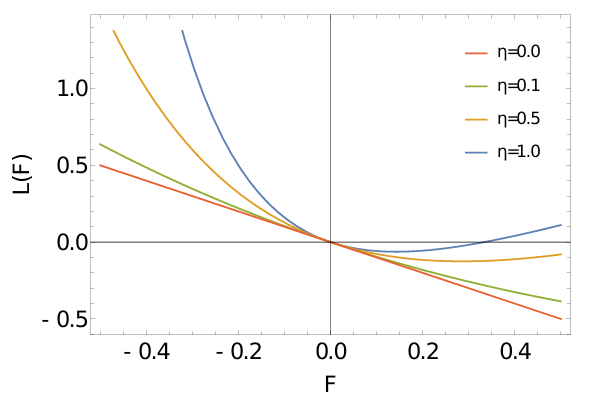
\includegraphics[width=0.7\textwidth]{fig/fig1.png}
    \caption{$\eta$ 取不同值时新NLE模型拉氏量 $L(F)$ 与 $F$ 的关系;取 $\gamma=1$}
\end{figure}   

\subsubsection{(2) 新NLE模型的物理对应}

利用电位移矢量 $\vec{D} $ 与 $\vec{E} $ 的关系 $\vec{D}=\partial L/\partial \vec{E} $,可由拉氏量式得到:

$$
\vec{D}
=\gamma\frac{1-7\eta F }{(1+\eta F)^3 } \vec{E}
$$

电位移矢量与电场可由电极化强度张量联系 $D_i = \varepsilon_i^{~~ j } E_j $ 

$$
\varepsilon_{ij} = \gamma \frac{1-7\eta F }{(1+\eta F)^3 }\delta_{ij} 
$$

类似地,磁场 $\vec{H}=-\partial L/\partial \vec{B} $ 结合拉氏量有

$$
\vec{H}
=\gamma \frac{1-7\eta F }{(1+\eta F)^3 } \vec{B}
$$

磁感强强度与磁场强度可由磁导率张量联系 $B_i=\mu_i^{~~j}H_j $,磁导率张量的逆 $\left(\mu^{-1} \right)_{ij} $

$$
\left(\mu^{-1} \right)_{ij}
=\gamma \frac{1-7\eta F }{(1+\eta F)^3 } \delta_{ij}
$$

可以认为新 NLE 拉氏量由这种特殊的介质生成。注意到 $\vec{D}\cdot\vec{H}\ne \vec{E}\cdot\vec{B}$,这违背了对偶对称性。

\subsubsection{(3) 场方程}

平坦时空中拉氏量给出欧拉-拉格朗日运动方程

$$
\partial_\mu\left(L_F F^{\mu\nu} \right) = 0
$$

其中,

$$
L_F
\equiv \frac{\partial L }{\partial F } 
=\frac{\gamma(-1+7\eta F) }{(1+\eta F)^3 }
$$
    
$F^{\mu \nu} $ 是麦克斯韦场强张量。运动方程可以回到无源麦克斯韦方程

$$
\nabla\cdot\vec{D} = 0,\quad
\frac{\partial \vec{D} }{\partial t } - \nabla\times\vec{H}= \vec{0} 
$$
    
由 Bianchi identity $\partial_\mu \tilde{F}^{\mu \nu}=0 $,$\tilde{F}^{\mu\nu}=\frac{1 }{2 } \varepsilon^{\mu\nu\rho\sigma}F_{\rho\sigma} $ 是电磁场张量的对偶张量,可得
    
$$
\nabla\cdot\vec{B} = \vec{0},\quad 
\frac{\partial \vec{B} }{\partial t } + \nabla\times\vec{E} = \vec{0} 
$$

\subsubsection{(4) 静电极限下点电荷产生的电场}

考虑静电极限(electrostatic limit) $\vec{B}=\vec{H}=\vec{0} $,点电荷产生的电位移矢量满足

$$
\nabla\cdot\vec{D} = e\delta(\vec{r})
$$

其解为

$$
\vec{D}
=\frac{e }{4\pi r^3 } \vec{r}
$$

结合 $\vec{D},\vec{E} $ 关系 $\vec{D}=\gamma\frac{1-7\eta F }{(1+\eta F)^3 }\vec{E} $ 和 $F=-E^2/2 $ 可得

$$
E+\frac{7 }{2 } \eta E^3
=\frac{e }{4\gamma \pi r^2 } \left(1-\frac{\eta  }{2 } E^2 \right)^3 
$$

上式限制 $F>-1/\eta$,且电场最大值为

$$
E_{\max}=\sqrt{\frac{2 }{\eta } }
$$

可见,新NLE模型中电场有限。当 $\eta\to 0 $,电场发散。

弱场极限 $\eta F\ll 1 $,$E(r) $ 可按 $\eta $ 展开

$$
E
=E_{(0)} + \eta E_{(1)} + \eta^2 E_{(3)} + \mathcal{O}\left(\eta^3 \right)
$$

$E_{(1)},E_{(2)} $ 分别代表对电场 $E_{(0)} $ 的一阶和二阶修正。比较系数可得
    
$$
E_{(0)}
=\frac{e }{4\pi\gamma r^2 }
$$

$$
E_{(1)} 
=-\frac{7 }{2 } E_{(0)}^3 - \frac{e }{4\pi \gamma r^2 } E_{(0)}^2
$$

$$
E_{(2)}
=-\frac{21 }{2 } E_{(0)}^2 E_{(1)} + \frac{e }{4\pi\gamma r^2 } \left(-3E_{(0)}E_{(1)} + \frac{3 }{4 } E_{(0)}^4 \right)
$$

弱场极限下,点电荷电场近似为

$$
E
\approx \frac{e }{4\pi\gamma r^2 } - 5\eta\left(\frac{e }{4\pi\gamma r^2 }  \right)^3 + \frac{273 }{4 } \eta^2\left(\frac{e }{4\pi\gamma r^2 }  \right)^5 + \mathcal{O}\left(\eta^3 \right)
$$

\begin{figure}
    \centering
    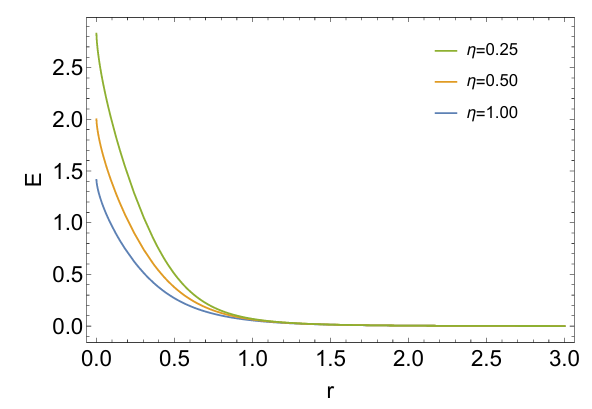
\includegraphics[width=0.7\textwidth]{fig/fig2.png}
    \caption{$\eta$ 取不同值时点电荷电场 $E$ 与 $r$ 的关系;取 $\gamma=1,e=1$}
\end{figure}   

\subsection{2. 点电荷的能量}

平坦时空中希尔伯特应力-能量张量(Hilbert stress-energy tensor)是一个对称张量且是不变量,其定义为

$$
T_{\mu\nu}^H
\equiv -\frac{2 }{\sqrt{-g} } \left(\frac{\partial \left(\sqrt{-g}L(F) \right) }{\partial g^{\mu\nu} }  \right)\bigg|_{g=\eta}
$$

结合新NLE模型 $L(F)=\frac{\gamma(3\eta F-1)F }{(1+\eta F)^2 } $ 可得

$$
T_{\mu\nu}^H
=\eta_{\mu\nu}L(F) - L_FF_\mu^\alpha F_{\nu\alpha}
$$

因此电能密度为

$$
\rho
=-T_t^t
=-L_FE^2-L(F)
=\frac{\gamma E^2\left[1+\frac{3 }{2 } \eta E^2 \left(4+\frac{\eta }{2 } E^2 \right) \right] }{2\left(1-\frac{\eta }{2 } E^2 \right)^3 } 
$$

总电能

$$
\epsilon
=4\pi\int_{0}^{+\infty} \rho(r)r^2\mathrm{d}r
$$

利用点电荷电场方程 $E+\frac{7 }{2 } \eta E^3=\frac{e }{4\gamma \pi r^2 } \left(1-\frac{\eta  }{2 } E^2 \right)^3 $,对 $r$ 的积分可转化为对 $E $ 的积分

$$
\epsilon
=\frac{e^{3/2} }{\sqrt{4\pi\gamma} } \int_{0}^{\sqrt{\frac{2 }{\eta  } }} \frac{\sqrt{\left(2-\eta E^2 \right)\left[4+3\eta E^2\left(8+\eta E^2 \right) \right]\left[4+\eta E^2\left(52+21\eta E^2 \right) \right]} }{16\sqrt{E}\left(2+7\eta E^2 \right)^{5/2} } \mathrm{d}E
$$

总能量有限,这与BI模型一致。当 $\eta\to 0$,点电荷自能发散。

\begin{figure}
    \centering
    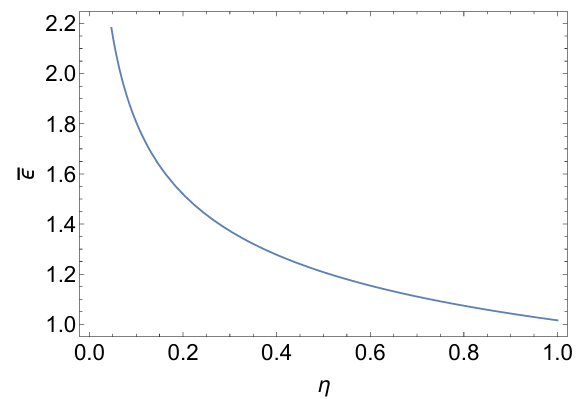
\includegraphics[width=0.7\textwidth]{fig/fig3.png}
    \caption{点电荷自能与 $\eta$ 的关系,反映点电荷自能有限性;$\bar{\varepsilon}=\varepsilon\sqrt{4\pi\gamma}/e^{3/2}$}
\end{figure}  

\subsection{3. 真空双折射}

考虑平面电磁波 $\left(\vec{e},\vec{b}\right) $ 沿 $z $ 轴在两片平行电容板间传播,$x $ 轴方向有匀强电场。外电场 $\bar{\vec{E}}=(\bar{E},0,0) $,总电场 $\vec{E}=\vec{e}+\bar{\vec{E}},\vec{B}=\vec{b} $,设 $\vec{e} $ 远小于 $\bar{\vec{E}} $,拉氏量

$$
L\left(\vec{e}+\bar{\vec{E}},\vec{b} \right)
=\gamma\frac{\left\{\frac{3 }{2 } \eta\left[\vec{b}^2-\left(\vec{e}+\bar{\vec{E}} \right)^2 \right] - 1 \right\}\left[\vec{b}^2-\left(\vec{e}+\bar{\vec{E}} \right)^2 \right] }{2\left\{1+\frac{\eta }{2 } \left[\vec{b}^2-\left(\vec{e} + \bar{\vec{E}}^2 \right) \right] \right\}^2 } 
$$

忽略高阶项,只保留二次项

$$
L^{(2)}(\vec{e}+\bar{\vec{E}},\vec{b})
=\frac{\gamma\eta\left(5+\frac{7 }{2 } \eta \bar{\vec{E}}^2 \right) }{\left(1-\frac{\eta }{2 } \bar{\vec{E}}^2 \right)^4 }\left(\vec{e}\cdot\bar{\vec{E}} \right)^2 - \frac{1 }{2 } \gamma \frac{\left(1+\frac{7 }{2 } \eta \bar{\vec{E}}^2 \right) }{\left(1-\frac{\eta }{2 } \bar{\vec{E}}^2 \right)^3 }\left(\vec{b}^2-\vec{e}^2 \right) 
$$

相应电位移矢量和磁场强度

$$
d_i = \frac{\partial L^{(2)} }{\partial e_i } = \left(\alpha\delta_i^j+\beta\bar{E}_i\bar{E}^j \right)e_j,\quad
h_i
=-\frac{\partial L^{(2)} }{\partial b_i } 
=\alpha\delta_i^j b_j 
$$

$$
\beta = \frac{2\gamma \eta\left(5+\frac{7 }{2 } \eta \bar{\vec{E}}^2 \right) }{\left(1-\frac{\eta }{2 } \bar{\vec{E}}^2 \right)^4 },\quad 
\alpha = \gamma \frac{\left(1+\frac{7 }{2 }\eta\bar{\vec{E}}^2 \right)  }{\left(1-\frac{\eta }{2 } \bar{\vec{E}}^2 \right)^3 }
$$

结合关系 $d_i=\varepsilon_i^j e_j,h_i=\left(\mu^{-1} \right)_i^j b_j $,对比可得
    
$$
\varepsilon_{ij} = \alpha\delta_{ij} + \beta\bar{E}_i\bar{E}_j ,\quad
\left(\mu^{-1} \right)_{ij} = \alpha\delta_{ij} 
$$

结合平面波麦克斯韦方程

$$
k_i d^i = k_i b^i = 0,\quad
\vec{k}\times\vec{e} = \omega\vec{b},\quad
\vec{k}\times\vec{h} = -\omega\vec{d} 
$$

得到电场 $\vec{e}$ 所满足的方程

$$
\left\{\varepsilon^{ijk}\varepsilon_{lmn} \left(\mu^{-1} \right)_k^l k_j k^m+\omega^2\epsilon_n^i \right\}e^n = 0
$$

$\varepsilon_{ijk} $ 是反对称张量。方程的矩阵形式为

$$
\Lambda \vec{e} = 0 
$$

其中,

$$
\Lambda
\equiv \begin{bmatrix}
-k^2 \alpha+\omega^2\left(\alpha+\beta\bar{E} \right) &0 &0 \\
0 &-k^2\alpha+\omega^2\alpha &0 \\
0 &0 &\omega^2\alpha
\end{bmatrix} 
$$

由 $\mathrm{det}(\Lambda)=0 $ 可知电场有两种模式。两种模式定义了色散关系。折射率定义为 $n\equiv k/\omega $,因此有两种不同的折射率

$$
n_\parallel = \sqrt{1+\frac{\beta }{\alpha } \bar{E}^2},\quad
n_\perp = 1 
$$

不同偏振的电磁波有不同的速度 $v_\parallel=n_\parallel^{-1},v_\perp=1 $,这里平行和垂直极化是相对于背景匀强电场而言的。这种真空双折射现象是由模型的非线性性造成的。当 $\eta\to 0$ 时,$\beta\to 0$,真空双折射现象也消失。

\subsection{4. 拉格朗日量的因果性和幺正性条件}

只有当因果性(causality)和幺正性(unitarity)成立时,NLE模型才是合理的\cite{shabad2011effective}。

若拉氏量满足不等式

$$
L_F \leq 0,\quad
L_{FF}\geq 0,\quad
L_F + 2F L_{FF} \leq 0
$$

则背景场上元激发的群速度不超过真空光速,且动能非负。

\subsubsection{(1) 电场部分的因果性和幺正性条件}

电场部分取 $B=0 $,拉氏量 $\displaystyle{L(F)=-\frac{\left(aF+1 \right)^m }{\delta(bF+1)^n } \left(\beta F \right)^p }$ ,前两个不等式给出

$$
n\geq m+1,\quad a\leq 0,\quad b\geq 0
$$

在此基础上,第三个不等式自动满足。

\subsubsection{(2) 磁场部分的因果性和幺正性条件}

磁场部分取 $E=0 $,类似可得

$$
n\geq m+1,\quad a\geq 0,\quad b\leq 0
$$

\subsubsection{(3) $n=m+1,a=-3b $ 时的因果性和幺正性条件}

此时拉氏量的偏微分为

$$
L_F
=\frac{\gamma\left(-1+7\eta F \right) }{\left(1+\eta F \right)^3 },\quad
L_{FF}
=\frac{2\gamma \eta\left(5-7\eta F \right) }{\left(1+\eta F \right)^4 } 
$$

$$
L_F + 2FL_{FF} 
=\gamma \frac{-\eta F\left(26-21\eta F \right) }{\left(1+\eta F \right)^4 }
$$

仅电场部分,取 $B=0 $,因果性和幺正性条件三个不等式给出
    
$$
-\frac{2+7\eta E^2 }{\left(2-\eta E^2 \right)^3 } \leq 0,\quad
\frac{10+7\eta E^2 }{\left(2-\eta E^2 \right)^4 } \geq 0,\quad
\frac{-4-\eta E^2\left(521\eta E^2 \right) }{\left(2-\eta E^2 \right)^4 } \leq 0
$$

所有情况要求 $E<\sqrt{2/\eta} $,而之前的结果表明 $E_{\max}=\sqrt{2/\eta} $,因此,对于所有 $E$ 的所有允许的取值,新NLE模型都满足因果性和幺正性条件。

分析磁场,取 $E=0 $,前两个不等式给出

$$
\left(-1+\frac{7 }{2 } \eta B^2 \right)\leq 0,\quad
\left(5-\frac{7 }{2 } \eta B^2 \right)\geq 0
$$

可以得到 $F<1/7\eta $。因此,只有当磁场的取值在一定范围内时,因果性条件才得到满足。

第三不等式给出

$$
-2+\eta B^2\left(26-\frac{21 }{2 } \eta B^2 \right)\leq 0
$$

得到 $(13-2\sqrt{37})/21<\eta F<(13+2\sqrt{37})/21 $。因此,对于纯磁场,只有一定范围内的磁场的取值才满足因果性和幺正性条件。

\subsection{5. 新NLE模型与广义相对论的耦合}

通过作用量把拉氏量 $L(F) $ 与引力进行最小耦合

$$
I
=\int \mathrm{d}^4 x\sqrt{-g}\left(\frac{R }{\kappa } + L(F) \right) 
$$

其中 $R $ 为里奇标量。变分可得运动方程

$$
\nabla_\mu\left(\frac{\partial L }{\partial F } F^{\mu\nu} \right)
=0,\quad
R_{\mu\nu} - \frac{1 }{2 } g_{\mu\nu} R
=\kappa T_{\mu\nu}
$$

其中 $R_{\mu\nu} $ 为里奇张量,$T_{\mu\nu} $ 为 Hilbert 能量-动量张量,在弯曲时空表达为

$$
T_\mu^\nu
=L\delta_\mu^\nu - L_F F_{\mu\lambda} F^{\nu \lambda}
$$

考虑球对称静态时空,线元

$$
\mathrm{d}s^2
=-f(r)\mathrm{d}t^2 + \frac{1 }{f(r) } \mathrm{d}r^2 + r^2\left(\mathrm{d}\theta^2+\sin^2\theta\mathrm{d}\phi^2 \right)
$$

假设仅 $F_{tr},F_{\theta\phi} $ 在 $F_{\mu\nu} $ 中非零,$F_{tr}=-F_{rt} $ 代表径向电场,$F_{\theta\phi}=-F_{\phi\theta} $ 代表径向磁场。应力能动-张量非零分量

$$
T_t^t = T_r^r
=L(F) - L_F F_{tr}F^{tr},\quad 
T_\theta^\theta
=T_\phi^\phi
=L(F) - L_F F_{\theta\phi}F^{\theta\phi}
$$

下面只关注纯磁场解和纯电场解。

\subsubsection{(1) 磁场正则黑洞解}

纯磁场解来自 $F_{tr=0} $,非零麦克斯韦张量分量 $F_{\theta\phi}=-q_m \sin\theta $,$q_m $ 为常数,可理解为一个磁单极子的总荷量,导致径向磁场 $B_r=q_m/r^2 $,麦克斯韦不变量 $F=q_m^2/2r^4 $;$r=0 $ 处奇异。

磁单极子能-动张量

$$
T_t^t
=T_r^r
=\frac{\gamma q_m^2\left(3\eta q_m^2-2r^4 \right) }{\left(2r^4+\eta q_m^2 \right)^2 }
$$

$$
T_\theta^\theta
=T_\phi^\phi
=\frac{\gamma q_m^2\left(4 r^8-2\eta q_m^2 r^4+3\eta^2q_m^4 \right) }{\left(2r^4+\eta q_m^2 \right)^3 }
$$

由线元可得爱因斯坦张量

$$
G_\mu^\nu
=\mathrm{diag}\left[\frac{f' }{r } + \frac{f-1 }{r^2 } ,\frac{f' }{r } + \frac{f-1 }{r^2 } , \frac{f'' }{2 } + \frac{f' }{r } , \frac{f'' }{2 } + \frac{f' }{r }  \right]
$$

$' $ 代表度规函数 $f(r) $ 的径向微分。爱因斯坦非线性麦克斯韦方程 $tt $ 或 $rr $ 分量简化为

$$
\frac{f' }{r } + \frac{f-1 }{r^2 } 
=\kappa \frac{\gamma q_m^2\left(3\eta q_m^2-2r^4 \right) }{\left(2r^4+\eta q_m^2 \right)^2 }
$$

解上面方程可得度规函数

$$
f(r)
=1+\frac{c_0 }{r } + \frac{\kappa \gamma q_m^2 r^2 }{2r^4+\eta q_m^2 } 
$$

$c_0 $ 是积分常数。取

$$
c_0=0,\quad
\gamma=-\frac{2b_0^2 }{\kappa q_m^2} ,\quad
\eta=\frac{2g^4 }{q_m^2 }
$$

$b_0,g $ 是长度量纲常数。线元可改写为

$$
\mathrm{d}s^2
=-\left(1-\frac{b_0^2r^2 }{r^4+g^4 }  \right)\mathrm{d}t^2 + \left(1-\frac{b_0^2r^2 }{r^4+g^4 }  \right)^{-1}\mathrm{d}r^2 + r^2\left(\mathrm{d}\theta^2+\sin^2\theta \mathrm{d}\phi^2 \right)
$$

当 $r$ 趋于无穷大,时空度规渐近平坦

$$
g_{tt}\to -1,g_{rr}\to 1 \quad \mathrm{as}\quad r\to\infty
$$

对于很小的 $r$,其行为与 de-Sitter 时空相似

$$
g_{tt}\to -\left(1-c^2r^2 \right),\quad g_{rr} \to \left(1-c^2r^2 \right)\quad \mathrm{as}\quad r\to 0
$$

$g_{tt}=0$ 给出黑洞视界的位置。若度规参数满足 $0<g<0.5 b_0^2 $,则上面几何代表一系列双视界黑洞;当 $g^2=0.5b_0^2$,得到单视界黑洞;若 $g^2>0.5b_0^2$,则黑洞没有视界。特别地,当 $g^2=0$,黑洞有一个视界。

\begin{figure}[htbp]
    \centering
    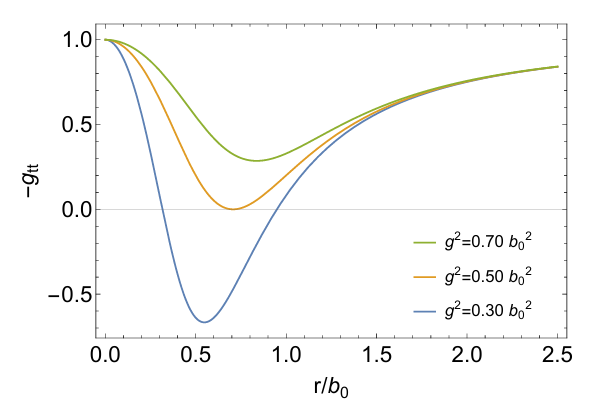
\includegraphics[width=0.5\textwidth]{fig/fig4.png}
    \caption{$g^2$ 取不同值时 $g_{tt}$ 与 $r$ 的关系}
\end{figure}  

可通过黎曼和里奇张量各分量是否发散来判断时空的正则性。坐标基底,非零黎曼曲率张量分量

$$
R^0_{~~ 110} 
=-\frac{b_0^2\left(3r^8 - 12 g^4 r^4 + g^8 \right) }{\left(r^4+g^4 \right)^3 } 
$$

$$
R^0_{~~220} = R^0_{~~330} = R^2_{~~112} = R^3_{~~113}
=\frac{b_0^2\left(r^4-g^4 \right) }{\left(r^4+g^4 \right)^2 }
$$

$$
R^3_{~~223}
=-\frac{b_0^2 }{r^4+g^4 } 
$$

里奇张量非零分量

$$
R_{00} = -R_{11} = -\frac{b_0^2\left(r^8-12g^4r^4+3g^8 \right) }{\left(r^4+g^4 \right)^3 } 
$$

$$
R_{22} = R_{33} = \frac{b_0^2 \left(3g^4-r^4 \right) }{\left(r^4+g^4 \right)^2 }
$$

当 $r\to 0 $,两个张量的分量都有限;当 $r\to \infty $,所有分量趋于零,这保证时空是渐进平坦的。

只有当曲率标量都是正则时时空才是正则的。因此考察三个标量不变量:
    
Ricci 标量

$$
R = g^{\mu\nu}R_{\mu\nu}
=\frac{4b_0^2\left(3g^8-5g^4r^4 \right) }{\left(r^4+g^4 \right)^3 }
$$

Ricci 收缩量

$$
R_{\mu\nu} R^{\mu\nu}
=\frac{4b_0^2 \left(r^{16}-14g^4r^{12}+74g^8r^8-30g^{12}r^4+9g^{16} \right) }{\left(r^4+g^4 \right)^6 }
$$

Kretschmann 标量

$$
K
=R_{\mu\nu\lambda\delta} R^{\mu\nu\lambda\delta}
=\frac{8\left(3g^{16}-10g^{12}r^4+74 g^8 r^8-34g^4r^{12}+7r^{16} \right)b_0^4 }{\left(r^4+g^4 \right)^6 }
$$

在 $r\to 0$ 时,三个不变量也都有限。 因此上述几何是正则的。

定义 $\rho=-T_t^t,\tau=t_r^r,p=T_\theta^\theta=T_\phi^\phi $

$$
\rho=-\tau
=\frac{b_0^2\left(3g^4-r^4 \right) }{\kappa \left(r^4+g^4 \right)^2 } 
$$

$$
p
=-\frac{b_0^2\left(3g^8-12g^4r^4+r^8 \right) }{\kappa \left(r^4+g^4 \right)^3 }
$$

Null Energy Condition(NEC)要求 $\rho+\tau \geq 0,\rho+p\geq 0 $,第一个不等式在 $\rho+\tau=0 $ 时自动满足;

$$
\rho+p
=\frac{2b_0^2 r^4\left(r^4-7g^4 \right) }{\kappa \left(r^4+g^4 \right)^3 }
$$

若第二个不等式得到满足,则只能 $r^4\leq 7g^4 $,即并非所有 $r$ 的取值都是合理的。

\subsubsection{(2) 裸电奇点解}

纯电场解 $B=0,F=-E^2/2,F_{\theta\phi}=0$,能-动张量的分量

$$
T_t^t = T_r^r
=L(F)-2F L_F 
=\frac{\gamma E^2\left(4+3\eta E^2\left(8+\eta E^2 \right) \right) }{\left(-2+\eta E^2 \right)^3 } 
$$

$$
T_\theta^\theta = T_\phi^\phi
=L(F)
=\frac{\gamma E^2\left(2+3\eta E^2 \right) }{\left(-2+\eta E^2 \right)^2 } 
$$

从爱因斯坦方程得到度规函数 $f(r)$ 满足

$$
\frac{f' }{r } + \frac{f-1 }{r^2 } = \frac{\gamma \kappa E^2 \left(4+3\eta E^2\left(8+\eta E^2 \right) \right) }{\left(-2+\eta E^2 \right)^3 }  
$$

$$
\frac{f'' }{2 } + \frac{f' }{r } = \frac{\gamma \kappa E^2\left(2+3\eta E^2 \right) }{\left(-2+\eta E^2 \right)^2 }  
$$

无法得到 $f(r)$ 的解析解,但在弱场极限 $\eta F\ll 1$ 下将 $f(r)$ 按 $\eta$ 展开

$$
f(r)
=1+\frac{c }{r }+\eta^0 f_{(0)} + \eta f_{(1)} + \eta^2 f_{(2)} + \mathcal{O}\left(\eta^3 \right) 
$$

代回原方程对比系数得

$$
\frac{f''_{(0)} }{2 } + \frac{f'_{(0)} }{r }
=\frac{\gamma \kappa }{2 } E_{(0)}^2   
$$

$$
\frac{f''_{(1)} }{2 } + \frac{f'_{(1)} }{r } 
=\frac{\gamma\kappa }{2 } \left(2E_{(0)}E_{(1)}+\frac{5 }{2 } E_{(0)}^4 \right) 
$$

$$
\frac{f''_{(2)} }{2 } + \frac{f'_{(2)} }{r }
=\frac{\gamma\kappa }{2 }\left(E_{(1)}^2+10E_{(0)}^3E_{(1)}+2E_{(0)}E_{(2)}+\frac{9 }{4 } E_{(0)}^6 \right)   
$$

相应度规函数的近似解为

$$
f(r)
=1+\frac{c }{r }+c_{(0)}\eta^0\frac{e^2 }{r^2 } + c_{(1)}\eta\frac{e^4 }{r^8 } + c_{(2)}\eta^2\frac{e^6 }{r^{10} } + \mathcal{O}\left(\eta^3 \right)   
$$

其中 $c_{(0)},c_{(1)},c_{(2)}$ 是任意常数。

为了在 $\eta$ 取任意值时数值求解度规函数,作变量替换 $\tilde{E}=E^2$,得到

$$
r\frac{\mathrm{d}f(r) }{\mathrm{d}r } + f(r)-1
=r^2\frac{\gamma \kappa\tilde{E}\left(4+3\eta\tilde{E}\left(8+\eta\tilde{E} \right) \right) }{\left(-2+\eta\tilde{E} \right)^3 }  
$$

此时把 $f(r)$ 看作 $\tilde{E}$ 的函数 $f(r)\to f(\tilde{E})$,对 $r$ 的微分转化为对 $\tilde{E}$ 的微分

$$
\frac{\mathrm{d}f }{\mathrm{d}\tilde{E} }\left(r\frac{\mathrm{d}\tilde{E} }{\mathrm{d}r }  \right) + f(\tilde{E})-1
=r^2\frac{\gamma\kappa\tilde{E}\left(4+3\eta\tilde{E}\left(8+\eta\tilde{E} \right) \right) }{\left(-2+\eta\tilde{E} \right)^3 }  
$$

进一步有

$$
\frac{4\tilde{E}\left(-2+\eta\tilde{E} \right)\left(2+7\eta\tilde{E} \right) }{4+\eta\tilde{E}\left(52+21\eta\tilde{E} \right) }\frac{\mathrm{d}f }{\mathrm{d}\tilde{E} } + f(\tilde{E})-1
=-\frac{e\kappa \sqrt{\tilde{E}}\left(4+3\eta\tilde{E}\left(8+\eta\tilde{E} \right) \right) }{16\pi\left(2+7\eta\tilde{E} \right) }   
$$

由于 $r\in[0,+\infty),\tilde{E}=E^2\in[0,2/\eta]$,则从上式可数值求解一定 $\eta$ 时 $f$ 与 $\tilde{E}$ 的关系。再结合 $\tilde{E}$ 与 $r$ 的关系就可以数值求解一定 $\eta$ 时度规函数 $f$ 与 $r$ 的关系。 

\begin{figure}[htbp]
    \centering
    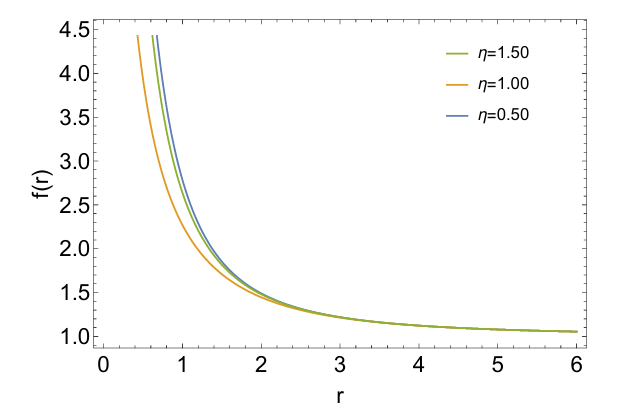
\includegraphics[width=0.7\textwidth]{fig/fig5.png}
    \caption{$\eta$ 取不同值时度规函数 $f(r)$ 与 $r$ 的关系;取 $e=2,\gamma=1/2\pi$}
\end{figure}  

为了确定时空是否有裸奇点,需要分析曲率标量的函数行为。

在球对称史瓦西规范度规中,三个独立的标量不变量可由度规函数及其微分表达。

Ricci 标量

$$
R
=g_{\mu\nu} R^{\mu\nu}
=\frac{4 }{r^2 } - \frac{4f(r) }{r^2 } - \frac{8f'(r) }{r } - 2f''(r) 
$$

通过变量替换 $\tilde{E}=E^2$ 可以写为

$$
R
=-8\kappa \left(L-FL_F \right)
=-\frac{8\gamma\kappa \eta\tilde{E}^2\left(10+3\eta\tilde{E} \right) }{\left(-2+\eta\tilde{E} \right)^3 }
$$

Ricci 收缩量

$$
R_{\mu\nu} R^{\mu\nu}
=8\left[\frac{f'(r) }{r } + \frac{f(r)-1 }{r^2 }  \right]^2 + 8 \left[\frac{f'(r) }{r } + \frac{f''(r) }{2 }  \right]^2
$$

$$
\begin{aligned}
    R_{\mu\nu} R^{\mu\nu}
    &=8\kappa\left[\left(L - 2FL_F \right)^2 + L^2 \right] \\
    &=\frac{16\kappa \gamma^2 \tilde{E}^2 \left\{16+\eta \tilde{E}\left[112+\eta\tilde{E}\left(296+3\eta \tilde{E}\left(20+3\eta\tilde{E} \right) \right) \right] \right\} }{\left(-2+\eta\tilde{E} \right)^6 }
\end{aligned}
$$

可见在 $\tilde{E}=2/\eta $ 或 $r=0$ 处三个标量发散,或者说 $r=0$ 是个时空奇点。可以计算,Kretschmann 标量 $R_{\mu\nu\lambda\delta}R^{\mu\nu\lambda\delta}  $ 在 $r=0$ 处也发散。因此,由拉氏量控制的非线性电单极子与爱因斯坦引力的耦合最小,导致了裸奇点。

\subsection{6. 小结}

\begin{itemize}

\item 模型构建与场方程

本文提出的新NLE模型在平直时空中表现出与麦克斯韦电动力学相似的极限行为,尤其是在弱场情况下。通过引入两个维度参数,模型能够限制点电荷的电场强度,使其在接近点电荷时达到一个有限的最大值,从而避免了自能量的发散。

通过求解场方程,本文展示了点电荷的电场强度随距离的变化,并通过幂级数展开和数值模拟验证了电场强度的有限性。

\item 真空双折射现象

在非线性电动力学中,光子在背景电磁场中的传播路径与麦克斯韦理论中的路径不同,表现出所谓的“真空双折射”现象。本文通过分析平面电磁波在均匀电场中的传播,展示了该模型中的真空双折射效应,并给出了相应的折射率表达式。

\item 因果性与幺正性条件

本文对提出的新NLE模型进行了因果性和幺正性条件的分析,确保模型在物理上是合理的。结果表明,该模型在所有背景电场下都满足因果性和幺正性条件,而在磁场情况下,仅在一定范围内满足这些条件。

\item 与广义相对论的耦合

本文将提出的新NLE模型与爱因斯坦的广义相对论(GR)进行最小耦合,研究了不同的时空解。结果表明,当源场为非线性磁单极子时,可以得到正则黑洞解;而当源场为点电荷时,则会导致裸奇点的出现。

通过分析曲率标量和能量条件,本文验证了正则黑洞的非奇异性,并指出裸奇点的存在是由于点电荷的电场在引力耦合下无法避免奇异性。

\item 结论与未来工作

本文提出的新NLE模型成功解决了麦克斯韦电动力学中点电荷的自能量发散问题,并在平直时空中表现出良好的物理性质。通过与广义相对论的耦合,模型能够生成正则黑洞解,但也揭示了裸奇点的存在。未来的研究可以进一步探索该模型在更广泛的参数范围内的引力耦合效应,尤其是研究双荷(dyonic)配置下的时空解,并分析这些解在天体物理学中的应用,如黑洞阴影和准正规模的计算。

\item 局限性

该模型在磁场情况下的因果性和幺正性条件仅在一定范围内成立。

当模型与广义相对论耦合时,虽然可以生成正则黑洞解,但源场本身仍然存在奇异性,表明时空奇点和场奇点之间的复杂关系仍需进一步研究。

\end{itemize}

\section{III. 非线性电动力学与黑洞}

\subsection{1. NLED形式}

假设非线性电磁场可由电磁势 $A_\mu$ 描述

$$
F_{\mu\nu}
=2A_{[\mu,\nu]}
$$

$F_{\mu\nu}$ 有一个不变量和一个伪不变量

$$
F = \frac{1 }{4 } F_{\alpha\beta}F^{\alpha\beta},\quad
\tilde{G} = \frac{1 }{4 } F_{\alpha\beta} \tilde{F}^{\alpha\beta} 
$$

其中 $\tilde{F}^{\alpha\beta}=\left(\mathrm{i}/2\sqrt{-g} \right)\varepsilon^{\alpha\beta\gamma\delta}F_{\gamma\delta}$ 是 $F^{\alpha\beta}$ 的对偶。

若 NLED 拉氏量在洛伦兹群作用下不变,则它依赖于 $F$ 和 $\tilde{G}$;同时,在弱场极限下应与经典线性理论相同。

\subsubsection{(1) $(F,\tilde{G})$ 和 $(P,\tilde{Q})$ 框架}

通过勒让德变换可以研究系统的正则形式。两个框架可通过勒让德变换联系。定义

$$
P^{\alpha\beta}
=2\frac{\partial L }{\partial F_{\alpha\beta} } 
=\frac{\partial L }{\partial F } F^{\alpha\beta} + \frac{\partial L }{\partial \tilde{G} } \tilde{F}^{\alpha\beta}
$$

哈密顿量定义为

$$
H
=\frac{1 }{2 } P^{\alpha\beta} F_{\alpha\beta} - L\left(F,G^2 \right)
$$

在 $(P,\tilde{Q})$ 框架里,哈密顿量依赖于两个新的不变量 $P,\tilde{Q}$

$$
P = \frac{1 }{4 } P_{\alpha\beta} P^{\alpha\beta},\quad
\tilde{Q} = \frac{1 }{4 } P_{\alpha\beta}\tilde{P}^{\alpha\beta}
$$

勒让德逆变换给出哈密顿方程

$$
F^{\alpha\beta}
=2\frac{\partial H }{\partial P_{\alpha\beta} } 
=\frac{\partial H }{\partial P } P^{\alpha\beta} + \frac{\partial H }{\partial Q } \tilde{P}^{\alpha\beta}
$$

此方程描述了电磁场张量 $F^{\alpha\beta}$ 如何依赖于动量张量 $P^{\alpha\beta}$ 和不变量 $P,Q$。

NLED 与引力耦合作用量

$$
S
=\int \mathrm{d}^4 x\sqrt{-g} \left\{R(16\pi)^{-1}-L \right\}
$$

$R $ 是曲率标量;$g:=\mathrm{det}\left|g_{\mu\nu} \right| $

$$
L
=\frac{1 }{2 } P^{\mu\nu}P_{\mu\nu} - H\left(P,\tilde{Q} \right)
$$

能动张量和曲率标量

$$
4\pi T_{\mu\nu}
=H_{,P} P_{\mu\alpha} P_\nu^\alpha - g_{\mu\nu}\left(2P H_{,P} + \tilde{Q} H_{,\tilde{Q}} - H \right)
$$

$$
R
=8\left(P H_{,P} + \tilde{Q} H_{,\tilde{Q}} - H \right) 
$$

其中,$\partial H/\partial P = H_{,P} $。曲率标量 $R$ 和能量-动量张量的迹可能不为零,这与麦克斯韦电动力学不同。

Born-Infeld 非线性电动力学由结构函数 $H(P,\tilde{Q}) $ 给出:

$$
H = b^2\left(1-\sqrt{1-2P/b^2+\tilde{Q}^2/b^4} \right) 
$$

其中,$b $ 是最大场强,是 BI 理论中的参数。

\subsubsection{(2) NLED能量条件}

利用类时矢量 $V^\alpha,V_\alpha V^\alpha<1 $ ,局域能量密度非负要求 $T_{\mu\nu}V^\mu V^\nu\geq 0 $;局域能流矢量非类空要求 $T_{\alpha\beta}T_\gamma^\alpha V^\beta V^\gamma\leq 0 $。这两个分别是弱能量条件(WEC)和主能量条件(DEC)。当下面的不等式得到满足时,这两个条件就得到满足

$$
H_{,P}>0,\quad
\left(P H_{,P} + \tilde{Q} H_{,\tilde{Q}} - H \right) \geq 0
$$

强能量条件(SEC)要求 $R_{\mu\nu}V^\nu V^\nu\geq 0 $,结合爱因斯坦方程得

$$
R_{\mu\nu}V^\mu V^\nu 
=8\left(T_{\mu\nu} V^\mu V^\nu + \frac{T }{2 }  \right) \geq 0
$$

需要注意,NLED物质可以违背SEC。

\subsection{2. NLED黑洞}

\subsubsection{(1) BI黑洞和EBIon}

静态球对称(SSS)线元

$$
\mathrm{d}s^2 = -\psi\mathrm{d}t^2 + \psi^{-1} \mathrm{d}r^2 + r^2\left(\mathrm{d}\theta^2+\sin^2\theta\mathrm{d}\phi^2 \right)
$$

HI发现一种解为\cite{hoffmann1937choice}

$$
\psi
=1-\frac{8\pi }{r } \int_{0}^{r} \left(\sqrt{r^4+1} - r^2 \right)\mathrm{d}r
$$

上面的解有锥形奇点;另一个正则解由场 $D_{,r}=1/r,E_{,r}=r^2/\left(r^4+1 \right) $ 给出,度规函数

$$
\psi_{HI}
=1-\frac{k }{r } + \frac{8\pi\gamma }{r } \int_{0}^{r} \left[r^2\ln\left(\frac{r^4 }{1+r^4 }  \right) \right] \mathrm{d}r
$$

对 SSS 线元,PT 发现\cite{pellicer1969nonlinear}

$$
\psi_{PT}
=1-\frac{d }{r } + \frac{8\pi }{r } \int_{0}^{r} H(x) x^2\mathrm{d}x
$$

点电荷电磁场

$$
F_{\mu\nu}
=-\frac{e }{r^2 } \frac{\partial H(P,0) }{\partial P } 2\delta_\mu^{[0}\delta_{\nu}^{r]}
$$

其中 $P=-e^2/4r^2$;若积分存在且有限,则当 $r\to 0$ 时电磁场张量是有限的;此外,当 $r$ 很大时,$H(P,0)\approx P$。这些条件保证了此解有较好的行为。

SSS 时空的 EBI 解由度规函数 $\psi_{BI}(r)$ 给出

$$
\Psi_{BI}(r)
=1-\frac{2m }{r } + \frac{2 }{3 } b^2\left(r^2-\sqrt{r^4+a^4} \right) + \frac{4g^2 }{3r } G(r)
$$

$$
G'(r)
=-\left(r^4+a^4 \right)^{-1/2}
$$

其中,$m$ 是质量参数,$g$ 是磁荷,$a^4=g^2/b^2$,$b$ 是 BI 模型参数。电磁场非零分量为

$$
F_{rt}
=g\left(r^4+a^4 \right)^{-1/2},\quad
P_{rt}
=\frac{g }{r^2 }
$$

黑洞解为

$$
G(r)
=\int_{r}^{\infty} \frac{\mathrm{d}s }{\sqrt{s^4+a^4} } 
=\frac{1 }{2a } \mathbb{F} \left[\arccos\left(\frac{r^2-a^2 }{r^2+a^2 }  \right) , \frac{1 }{\sqrt{2} }  \right]
$$

其中,$\mathbb{F}$ 是第一类椭圆积分。这个解在 $r=0$ 处发散。另一方面,类粒子解(所谓的 EBIon 解)为

$$
G(r)
=\int_{0}^{r} \frac{-\mathrm{d}s }{\sqrt{s^4+a^4} } 
=-\frac{1 }{2a } \mathbb{F}\left[\arccos\left(\frac{a^2-r^2 }{a^2+r^2 } , \frac{1 }{\sqrt{2} }  \right) \right]
$$

这个解在 $r=0$ 处有限。

二者的联系为

$$
\int_r ^{\infty} \frac{\mathrm{d}s }{\sqrt{s^4+a^4} } + \int_0^r \frac{\mathrm{d}s }{\sqrt{s^4+a^4} } 
=\frac{1 }{a } \mathrm{K}\left[\frac{1 }{2 }  \right] 
$$

其中,$\mathrm{K}\left[\frac{1 }{2 } \right]$ 是第一类完全椭圆积分。在 $r$ 很大时,解趋于 RN 解;当 BI 模型参数 $b\to\infty$,得到线性电磁场 RN 解;在无电荷极限 $b=0$ 下,得到史瓦西黑洞解。

\begin{figure}
    \centering
    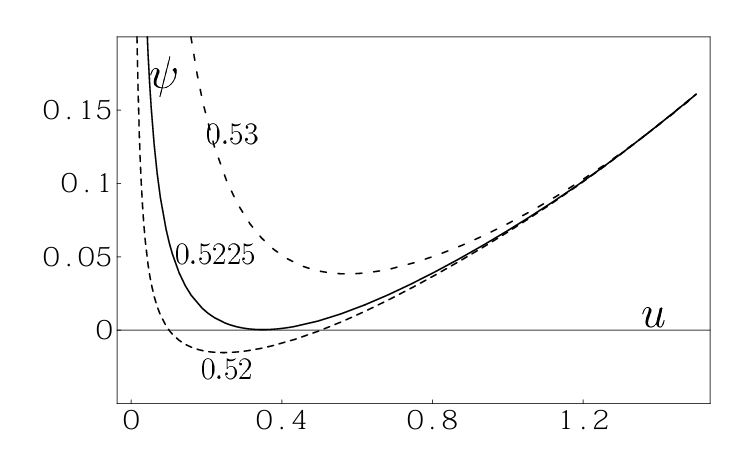
\includegraphics[width=0.4\textwidth]{fig/fig6.png}
    \caption{$bm$ 取不同值时BI度规函数 $\psi$ 与 $u=r/m$ 的关系;$\psi(r_\Delta)=0$ 给出视界的位置}
\end{figure}

\subsubsection{(2) BI黑洞中测试粒子的轨迹}

测试粒子运动过程中有两个守恒量:能量 $E$ 和角动量 $l$;若把粒子运动限制在赤道面 $\theta=\pi/2$ 上,则可用有效势进行分析。

对于有质量测试粒子,其轨迹由洛伦兹方程给出

$$
\frac{\mathrm{d}^2 x^\nu }{\mathrm{d}\tau^2 } + \Gamma_{\alpha\beta}^\nu \frac{\mathrm{d}x^\alpha }{\mathrm{d}\tau } \frac{\mathrm{d}x^\beta }{\mathrm{d}\tau } 
=-\frac{\varepsilon }{\mu } F_{\sigma}^{\nu} \mathrm{d}x^\sigma \mathrm{d}\tau
$$

其中,$\varepsilon$ 是电荷量,$\mu$ 是质量,$\tau$ 是沿轨迹的仿射参数。利用两个守恒量可得

$$
\dot{r}^2 + \psi\left(\frac{l^2 }{r^2 } + 1 \right) - \left\{E+\frac{\varepsilon g }{\mu } \sqrt{\frac{b }{4g } } \mathbb{F} \left[\arccos\left(\frac{r^2-g/b }{r^2+g/b }  , \frac{1 }{\sqrt{2} }  \right) \right] \right\}^2=0
$$

与 $\dot{r}^2/2+U_{\mathrm{eff}}(E,l,r)=0$ 比较可得有效势。对于光子,类似有

$$
\dot{r}_{ph}
=\sqrt{E^2 - \frac{\Psi_{BI} l^2 }{r^2 } \left(1+\frac{a^4 }{r^4 }  \right)^{-1}} 
$$

可以发现 $(\mathrm{d}r/\mathrm{d}t)_{\mathrm{photon}}<(\mathrm{d}r/\mathrm{d}t)_{\mathrm{grav}}$,即非线性效应导致光的传播速度小于引力波的传播速度。这可以解释为光子在电介质中传播导致的。

\begin{figure}[htbp]
    \centering
    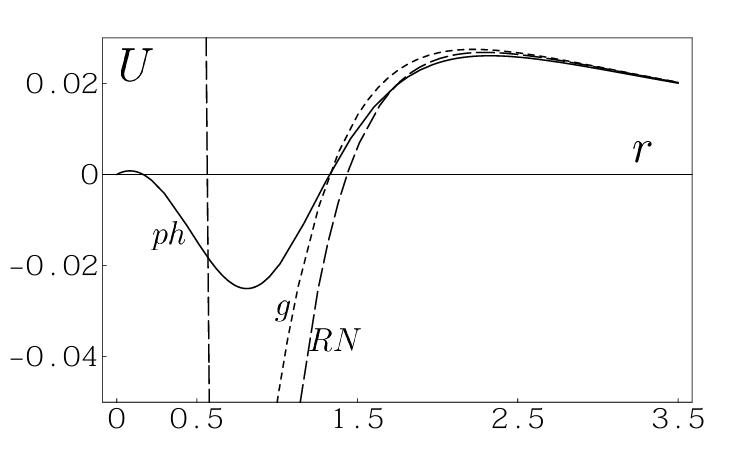
\includegraphics[width=0.7\textwidth]{fig/fig7.png}
    \caption{无质量粒子的有效势;g代表零测地线,ph代表BI光子;取 $g=0.6,b=0.75,l=1$}
\end{figure}

\subsection{3. NLED黑洞热力学}

考虑静态球对称黑洞,热力学第一定律给出

$$
\delta M_{\Delta} = \frac{\kappa }{8\pi } \delta a_{\Delta} + \Phi_\Delta \delta Q_\Delta
$$

其中,$\kappa$ 为视界处的表面引力,$M_\Delta$ 为视界质量,$a$ 为视界面积,$Q$ 为电荷,$\Phi$ 为电势;另一方面,Smarr 公式给出

$$
M_\Delta = \frac{\kappa a_\Delta }{4\pi } + \Phi_\Delta Q_\Delta
$$

Rasheed 发现,对于非线性电动力学,上面公式不适用。但可以认为

$$
M_\Delta = \frac{\kappa a_\Delta }{4\pi } + \Phi_\Delta Q_\Delta + V\left(a_\Delta , Q_\Delta , P_\Delta \right)
$$

其中,$V$ 是由视界参数决定的未知势。

Bardeen模型\cite{ayon2000bardeen}是爱因斯坦场方程与一种特定非线性电动力学耦合的准确解,其拉氏量为

$$
\mathcal{L}(F)
=\frac{2 }{2 sg^2 } \left(\frac{2g^2 F }{1+\sqrt{2g^2 F} }  \right)^{5/2}
$$

其中,$g$ 是磁荷,$F$ 是电磁场不变量,$s=g/m$;对于 SSS 时空,相应度规函数为

$$
\psi_B
=1-\frac{2 m(r) }{r } 
=1-\frac{2mr^2 }{\left(r^2+g^2 \right)^{3/2} }
$$

Bardeen 解不含电荷,视界质量只依赖于视界面积

$$
M_\Delta
=\frac{1 }{8\pi } \int\kappa \mathrm{d}a
=\int \left(1-m' \right)\mathrm{d}r
$$

视界质量的正号性给出 $m(r)\leq r$,且 $\psi_B\geq 0$,这导致 $(r^2+g^2)^3\geq 4m^2 r^4$;$g^2=16m^2/27$ 对应极端黑洞;$g^2<16m^2/27$ 时存在内外事件视界。

Bardeen 黑洞的势 $V$ 是不确定的,除非把一个积分常数设为零,于是
    
$$
V = m r^3 \frac{2g^2 - r^2 }{\left(g^2 + r^2 \right)^{3/2} }
$$

代入 Smarr 公式得到

$$
M_\Delta = \frac{r }{2 } - \frac{m r^3 }{\left(r^2+g^2 \right)^{3/2} } 
$$

注意到,Bardeen 黑洞的视界质量只依赖于视界面积,这是因为磁荷被认为是视界的不变参数。

\begin{figure}[htbp]
    \centering
    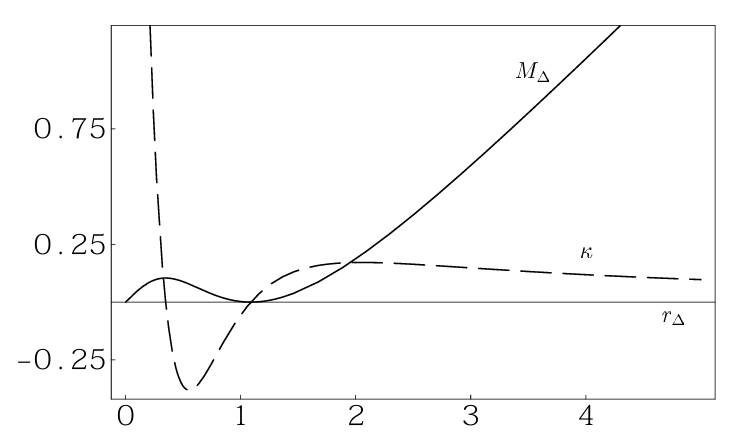
\includegraphics[width=0.4\textwidth]{fig/fig8.png}
    \caption{极端Bardeen黑洞视界质量 $M_\Delta$ 和表面引力 $\kappa$ 与视界半径 $r_\Delta$ 的关系;取 $g^2=16m^2/27 $}
\end{figure}

\subsection{4. 孤立视界框架和质量关系}

ADM模型中,带毛黑洞(hairy black hole)可以被视为普通黑洞和孤立子的束缚态。下面的公式将有色黑洞解的视界质量与相应理论的孤立子解的ADM质量联系起来\cite{ashtekar2000isolated}

$$
M_{\mathrm{sol}}^{(n)} = M_{\mathrm{ADM}}^{(n)} - M_\Delta^{(n)} 
$$

若EBI理论给出两个确定解:黑洞解和孤子解,那么即使 EBI 黑洞是无色的(is not a coloured one),我们也应当采用 ACS 模型,认为 $b$ 是一个自由参数。因此这里 $n$ 应该替换为 BI 参数 $b$(分立或连续)。 

EBI 解中,视界质量和 ADM 质量是视界半径 $r_\Delta$ 的函数,它们分别为

$$
M_\Delta^{(b)}(r_\Delta)
=\frac{r_\Delta }{2 } + \frac{b^2 r_\Delta }{3 } \left(r_\Delta^2 - \sqrt{r_\Delta^4 + a^4} \right) - \frac{2g^2 }{3 } \int_0^{r_\Delta} \frac{\mathrm{d}s }{\sqrt{a^4+s^4} } 
$$

$$
M_{\mathrm{ADM}}^{(b)}(r_\Delta)
=\frac{r_\Delta }{2 } + \frac{b^2 r_\Delta }{3 } \left(r_\Delta^2 - \sqrt{r_\Delta^4 + a^4} \right) + \frac{2g^2 }{3 } \int_{r_\Delta}^{\infty} \frac{\mathrm{d}s }{\sqrt{a^4+s^4} }
$$

\begin{figure}[htbp]
    \centering
    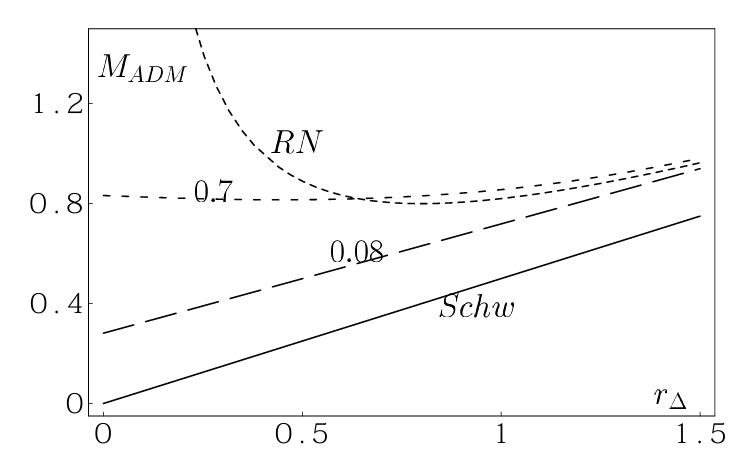
\includegraphics[width=0.5\textwidth]{fig/fig9.png}
    \caption{AMD质量作为视界半径 $r_\Delta$ 的函数;BI参数取 $b=0.7$ 和 $b=0.08$}
\end{figure}

\begin{figure}[htbp]
    \centering
    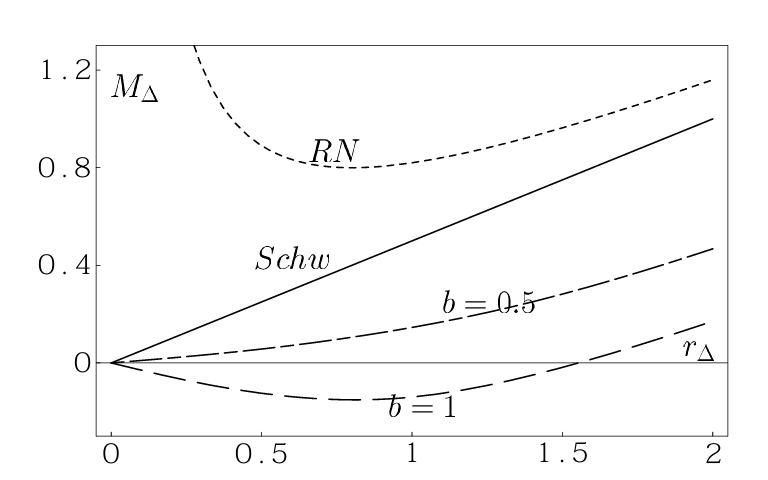
\includegraphics[width=0.5\textwidth]{fig/fig10.png}
    \caption{视界质量作为视界半径 $r_\Delta$ 的函数;BI参数取 $b=0.5$ 和 $b=1$;注意到 $M_{\Delta}^{\mathrm{RN}}>M_{\Delta}^{\mathrm{Schw}}>M_{\Delta}^{\mathrm{BI}}$}
\end{figure}

由于大多数 ACS 特征得到了满足,可以认为,当保持电荷不变而变化 BI 参数 $b$ 时,EBI 理论的静态部分可以用 Ashtekar 等人提出的有色黑洞(colored black hole)的启发式(heuristic)模型来描述。

\subsection{5. NLED黑洞的稳定性}

稳定性条件是一些对拉氏量及其微分 $L(F),L_F,L_{FF}$ 的约束\cite{moreno2003stability}。变量替换 $y=\sqrt{2g^2 F}$ 后可表述为
$$
L(y)>0,\quad
L(y)_{,y}>0,\quad
L(y)_{,yy}>0 
$$

$$
f(y)
\equiv yL_{,yy} / L_{,y} > 0,\quad
f(y) N(y) < 3    
$$

其中,$N(y)$ 为 SSS 线元度规函数。BI 拉氏量满足稳定性条件。把 BI 拉氏量写作 $y$ 的函数,取 $\tilde{G}=0$ 得

$$
L(y)
=b^2\left(\sqrt{1+\frac{y^2 }{b^2 g^2 } } - 1 \right) > 0 
$$

其他不等式

$$
L_{,y} = \frac{y }{g^2 } \left(1 + \frac{y^2 }{b^2 g^2 }  \right)^{-1/2} > 0
$$

$$
L_{,yy} = \frac{1 }{g^2 } \left(1 + \frac{y^2 }{b^2 g^2 }  \right)^{-3/2} > 0
$$

$$
f(y) = y\frac{L_{,yy} }{L_{,y} } = \left(1 + \frac{y^2 }{b^2 g^2 }  \right)^{-1} > 0
$$

对于所有 $y$,以上不等式均成立。考虑不等式 $f(y)N(n)<3$,由于 $0<f(y)\leq 1$,则其化简为 $\psi_{BI}(y)<3$

对于黑洞情况,度规函数

$$
\psi_{BI}(y)
=1-\frac{2m\sqrt{y} }{g } + \frac{2b^2 g^2 }{3y } \left(1-\sqrt{1+\frac{y^2 }{b^2 g^2 } } \right) + \frac{2\sqrt{gby} }{3 } \mathbb{F}\left[\arccos\left(\frac{gb-y }{gb+y } \right), \frac{1 }{\sqrt{2} }   \right] 
$$

在 $0<y<y_\Delta=8.35$ 范围内,$0<\psi_{BI}(y)\leq 1$,不等式得以满足。

对于 EBI 方程类粒子解,度规函数

$$
\psi_{BI}(y)
=1-\frac{2m\sqrt{y} }{g } + \frac{2b^2 g^2 }{3y } \left(1-\sqrt{1+\frac{y^2 }{b^2 g^2 } } \right) - \frac{2\sqrt{gby} }{3 } \mathbb{F}\left[\arccos\left(\frac{y-gb }{gb+y } \right), \frac{1 }{\sqrt{2} } \right]
$$

$N(y=0)=1$,而 $N(y)$ 单调递减,因此 $N=\psi<3$ 总能满足。

因此,EBI 的黑洞解和类粒子解都是稳定的。

\subsection{4. 小结}

\begin{itemize}
    \item NLED形式化框架

本文首先回顾了非线性电动力学的形式化框架,特别是基于电磁场不变量 $F$ 和 $\tilde{G}$ 的拉格朗日量 $L(F,\tilde{G})$ 及其通过勒让德变换得到的哈密顿量 $H(P,\tilde{Q})$。接着讨论了非线性电动力学与广义相对论耦合下的黑洞解,特别是Born-Infeld黑洞的解及其性质。
    \item NLEd黑洞解
    
    Born-Infeld黑洞的解在静态球对称时空下具有以下形式
$$
\Psi_{BI}(r)
=1-\frac{2m }{r } + \frac{2 }{3 } b^2\left(r^2-\sqrt{r^4+a^4} \right) + \frac{4g^2 }{3r } G(r)
$$

$$
G'(r)
=-\left(r^4+a^4 \right)^{-1/2}
$$

该解在无穷远处趋于RN解,在近场区域($r\to 0$)表现出正则性,避免了经典电磁理论中的奇点问题。
    \item NLED黑洞热力学

    本文还讨论了非线性电动力学黑洞的热力学性质,特别是第一定律和Smarr公式的推广形式。在非线性电动力学中,由于质量函数不再具有齐次性,传统的Smarr公式需要进行修正,引入一个额外的势函数 $V$ 来描述黑洞的质量与电荷、面积等参数之间的关系。

    \item NLED黑洞稳定性分析

    本文进一步分析了BI黑洞的稳定性。通过线性扰动理论,作者证明了BI黑洞在满足一定条件下是稳定的。特别是,BI拉格朗日量及其导数满足一系列不等式,确保了黑洞解在外部通信区域(DOC)内的稳定性。
\end{itemize}

\section{IV. f(T)引力框架下的非线性电动力学与广义热力学第二定律}

\subsection{1. f(T)引力和NLED基础}

\subsubsection{(1) 广义Teleparallel引力}

$f(T)$ 引力中的基本元素是四分量场 $h_a(x^\mu)$,其中英文字母标记切空间,希腊字母标记时空。$h_a=h_a^\mu\partial_\mu$,分量满足

$$
h_\mu^a h_b^\mu = \delta_b^a,\quad h_\mu^a h_a^\nu = \delta_\mu^\nu.
$$

其与度规张量 $g_{\mu\nu}$ 的关系为 $ g_{\mu\nu}=\eta_{ab}h_\mu^ah_\nu^b$,其中 $\eta_{ab}=\mathrm{diag}(1,-1,-1,-1)$ 是切空间中的闵氏度规。借助魏森博克联络 $\Gamma_{~~\mu\nu}^{\lambda}=h_a^\lambda \partial_\nu h_\mu^a$,扭率张量 $T^\rho_{~~\mu\nu}$ 和张量 $S_\rho^{~~\mu\nu}$ 可定义为

$$
T^{\lambda}_{~~\nu\mu} = \Gamma^\lambda_{~~\nu\mu} - \Gamma^\lambda_{~~\mu\nu} = h_a^\lambda\left(\partial_\nu h_\mu^a - \partial_\mu h_\nu^a \right),
$$

$$
S_\rho^{~~\mu\nu} = \frac{1 }{2 } \left(K^{\mu\nu}_{~~~~\rho} + \delta_\rho^\mu T^{\theta\nu}_{~~~~\theta} - \delta_\rho^\nu T^{\theta\mu}_{~~~~\theta} \right),
$$

其中,$K^{\mu\nu}_{~~~~\rho}=-\frac{1}{2}(T^{\mu\nu}_{~~~~\rho}-T^{\nu\mu}_{~~~~\rho}-T^{\mu\nu}-T_\rho^{~~\mu\nu}) $。$f(T)$ 引力的作用量

$$
S = \frac{1}{2\kappa^2}\int \mathrm{d}^4 x [ef(T)+L_m]
$$

其中,$e=\sqrt{-g},\kappa^2=8\pi G$,$G$ 是引力常量,$L_m$ 是宇宙中物质拉格朗日密度。对作用量变分可得场方程

$$
\left[e^{-1}\partial_\mu \left(e S_a^{~~\mu\nu} + h_a^\lambda T^\rho_{~~\mu\lambda} S_\rho^{~~\nu\mu} \right) \right] f_T + S_a^{~~\mu\nu} \partial_\mu(T) f_{TT} + \frac{1 }{4 } h_a^\nu f
=\frac{1 }{2 } \kappa^2 h_a^\rho T_\rho^\nu
$$

其中,$f_T=\mathrm{d}f/\mathrm{d}T,f_{TT}=\mathrm{d}^2f/\mathrm{d}T^2$,$T_\rho^\nu$ 是理想流体的能-动张量。平坦 FRW 宇宙线元

$$
\mathrm{d}s^2
=\mathrm{d}t^2 - a^2(t)\left(\mathrm{d}x^2+\mathrm{d}y^2+\mathrm{d}z^2 \right),
$$

其中,$a$ 是依赖于时间的尺度因子,相应 $h_\mu^a=\mathrm{diag}(1,a,a,a)$。修改 Friedmann 方程描述了宇宙的演化

$$
12 H^2 f_T + f = 2\kappa^2 \rho_t,
$$

$$
48H^2\dot{H} f_{TT} - \left(12 H^2 + 4\dot{H} \right) f_T - f= 2\kappa^2 p_t,
$$

其中,$H=\dot{a}/a$ 是哈勃参数,$\rho_t,p_t$ 是宇宙的总能量密度和压力。

\subsubsection{(2) 非线性电动力学}

对任意物理量 $Y$,体积空间平均值定义为

$$
\bar{Y}
=\lim_{V\to V_0} \frac{1 }{V } \int Y\sqrt{-g} \mathrm{d}^3 x,
$$

其中,$g$ 是度规行列式,$\displaystyle{V=\int\sqrt{-g}\mathrm{d}^3 x } $,电场和磁场的平均值

$$
\bar{E}_i = 0,\quad
\bar{B}_i = 0,\quad
\overline{E_i B_i} = 0,\quad
\overline{E_i E_j} = -\frac{1 }{3 } E^2 g_{ij},\quad
\overline{B_i B_j} = -\frac{1 }{3 } B^2 g_{ij},
$$

利用电磁场不变量 $F,F^*$ 来表达拉氏量,保留至二阶

$$
\mathcal{L}=-\frac{1 }{4 } F + \omega F^2 + \eta_0 F^{*2},
$$

其中,$F=F_{\mu\nu} F^{\mu\nu}=2(B^2-E^2),F^*=F_{\mu\nu}^*F^{\mu\nu}=-4\vec{E}\cdot\vec{B}$,$\omega_0,\eta_0$ 是任意常数。相应能-动张量

$$
T_{\mu\nu}
=-4\mathcal{L}_F F_\mu^{~~\alpha} F_{\alpha\nu} + \left(F^* \mathcal{L}_{F^*} - \mathcal{L} \right) g_{\mu\nu},
$$

结合电磁场平均值以及理想流体 $T_{\mu\nu}=(\rho+p)u_\mu u_\nu-p g_{\mu\nu}$,可得能量密度 $\rho$ 和压力 $p$

$$
\rho = -\mathcal{L} - 4E^2 \mathcal{L}_F,
$$

$$
p = \mathcal{L} + \frac{4 }{3 } \left(E^2-2B^2 \right)\mathcal{L}_F,
$$

考虑等离子体中迅速衰减至零的电场,进一步有

$$
\rho_B = \frac{1 }{2 } B^2\left(1-8\omega B^2 \right),
$$


$$
p_B = \frac{1 }{6 } B^2 \left(1-40\omega_0 B^2 \right),
$$

当 $\omega_0=\eta_0=0$ 时,拉氏量退化为线性麦克斯韦拉氏量,能动张量也退化

$$
\mathcal{L} = -\frac{1 }{4 } F,\quad
T_{\mu\nu} = F_\mu^{~~\alpha} F_{\alpha\nu} + \frac{1 }{4 } F g_{\mu\nu}.
$$

对于非线性过程

$$
\rho = 3p = \frac{1 }{2 } \left(E^2 + B^2 \right),
$$

这表明宇宙由普通辐射组成,具有正压力。

\subsection{2. 宇宙学参数和热力学}

修改 Friedmann 场方程可写为

$$
\frac{3 H^2 }{\kappa^2 } = \rho_t,\quad
-\frac{2\dot{H} }{\kappa^2 }  = \rho_t + p_t,
$$

其中,$\rho_t=\rho_m+\rho_B+\rho_T,p_t=p_m+p_B+p_T$,下标 $m,B,T$ 分别代表物质,磁场和扭率的贡献。

$$
\rho_T = \frac{1 }{2\kappa^2 } \left(-12 H^2 f_T - f + 6H^2 \right),
$$

$$
p_T = -\frac{1 }{2\kappa^2 } \left[48\dot{H}H^2 f_{TT} - \left(12 H^2 + 4\dot{H} \right) f_T - f + 6 H^2 + 4\dot{H} \right],
$$

为了方便,取 $p_m=0$,能量守恒方程

$$
\dot{\rho}_m + 3H \rho_m = 0,
$$

$$
\dot{\rho}_B + 3H\left(\rho_B + p_B \right) = 0,
$$

$$
\dot{\rho}_T + 3H\left(\rho_T + p_T \right) = 0,
$$

第一条方程解得

$$
\rho_m = \rho_{m0} a^{-3},
$$

其中,$a_{m0}$ 是任意常量。第二条方程解得

$$
B=\frac{B_0}{a^2},
$$

其中,$B_0$ 是任意常数。这表明磁场能量密度的演化随宇宙的膨胀而衰减。

EoS(equation of state)参数

$$
\begin{aligned}
    \omega_t
    &=\left\{-\frac{1 }{\kappa^2 } \left[48\dot{H}H^2 f_{TT} - \left(12 H^2 + 4\dot{H} \right) f_T - f + 6 H^2 + 4\dot{H} \right] + \frac{B^2 }{6 } \left(1-40\omega_0 B^2 \right) \right\} \\
    &\times \left\{\rho_{m0} a^{-3} + \frac{1 }{2\kappa^2 } \left[6 H^2 - f-12 H^2 f_T \right] + \frac{B^2 }{2 } \left[1-8\omega_0 B^2 \right] \right\}^{-1}
    \end{aligned}
$$

减速参数 $q$ 是宇宙膨胀加速度的度量,其由下式给出

$$
q = -1 - \frac{\dot{H} }{H^2 } .
$$

负的 $q$ 意味着加速状态。

当前情况下 $q_t=\frac{1}{2}(1+3\omega_t)$,于是
$$
\begin{aligned}
    2q_t
    &=1 + 3\left[-\frac{1 }{\kappa^2 } \left(48\dot{H} H^2 f_{TT} - \left(12 H^2 + 4\dot{H} \right) f_T - f + 6H^2 + 4\dot{H} \right) + \frac{B^2 }{6 } \left(1-40\omega_0 B^2 \right) \right] \\
    &\times \left[\rho_{m0}a^{-3} + \frac{1 }{2 } \left(6H^2-f-12H^2 f_T \right) + \frac{B^2 }{2 } \left(1-8\omega_0 B^2 \right) \right]^{-1}
\end{aligned}
$$

这是 $f(T)$ 的EoS(Equation of State),可以通过几个 $f(T)$ 模型来检查这些宇宙学参数的行为。

GLST说,在视界里和视界上的总熵不随时间减少。

由热力学第一定律有克劳修斯关系 $-\mathrm{d}E=T_X\mathrm{d}S_X$,其中 $S_X=A/(4G)$ 是 Bekenstein 熵,$A=4\pi R_X^2$ 是视界面积,$X$ 是任意视界,$T_X=1/(2\pi R_X)$ 是霍金温度。Miao 等人发现在 $f(T)$ 引力中热力学第一定律被违背,这导致额外的熵增项 $S_P$;而在 $f_{TT}$ 很小时,热力学第一定律成立,这时熵 $S_X=(Af_T)/(4G)$,而与 $S_P$ 无关。下面采用更一般的方法来研究磁 $f(T)$ 场景下的 GSLT。熵对时间微分

$$
\frac{\mathrm{d}S_X }{\mathrm{d}t } + \frac{\mathrm{d}S_P }{\mathrm{d}t } = \frac{\pi R_X }{G } \left(2\dot{R}_X f_T + R_X\dot{T} f_{TT} \right).
$$

利用吉布斯方程找到视界熵正常熵(normal entropy) $S_I$ 的变化率

$$
\frac{\mathrm{d}S_I }{\mathrm{d}t } 
=\frac{1 }{T_X } \left(\frac{\mathrm{d}E_I }{\mathrm{d}t } + p_t\frac{\mathrm{d}V }{\mathrm{d}t }  \right),
$$

其中,$E_I=\rho_t V,V=4\pi R_X^3/3$ 是视界体积。计算得

$$
\frac{\mathrm{d}S_I }{\mathrm{d}t } 
=\frac{4\pi R_X^2 }{T_X } \left(\dot{R}_X - H R_X \right)\left(\rho_t+p_t \right).
$$

总熵对时间的微分

$$
\begin{aligned}
    &\frac{\mathrm{d}S_X }{\mathrm{d}t } + \frac{\mathrm{d}S_P }{\mathrm{d}t } + \frac{\mathrm{d}S_I }{\mathrm{d}t } \\
    =&\frac{\pi R_X }{G } \bigg\{2\dot{R}_X f_T + R_X\dot{T}f_{TT} \\
    &+ 8\pi G R_X^2 \left[\rho_{m0}a^{-3} + \frac{1 }{\kappa^2 } \left(4\dot{H} T f_{TT} + 2\dot{H}\left(f_T-1 \right) \right) + \frac{2B_0^2 }{3a^4 } \left(1-\frac{16\omega_0 B_0^2 }{a^4 }  \right) \right] \\
    &\times \left[\dot{R}_X - H R_X \right] \bigg\}
\end{aligned}
$$

GSLT认为 $(\dot{S}_X+\dot{S}_I+\dot{S}_P)\geq 0$,下面讨论两种常用的宇宙学视界:哈勃视界(Hubble Horizon)和事件视界(Event Horizon)。

\subsubsection{(1) 哈勃视界}

假设FRW宇宙热力学系统的边界被处于平衡状态的表观视界(apparent horizon)占据。对于平坦的 FRW,它退化为半径为 $R_H$ 的哈勃视界

$$
R_H = \frac{1 }{H } ,\quad
\dot{R}_H = -\frac{\dot{H} }{H^2 }
$$

把任意视界 $X$ 替换为 $H$ 得

$$
\begin{aligned}
    &\frac{\mathrm{d}S_X }{\mathrm{d}t } + \frac{\mathrm{d}S_P }{\mathrm{d}t } + \frac{\mathrm{d}S_I }{\mathrm{d}t } \\
    =&-\frac{\pi }{G H} \bigg\{\frac{2\dot{H} }{H^2 } f_T + 12\dot{H}f_{TT} +\frac{8\pi G }{H^2 }\left(1+\frac{\dot{H} }{H^2 }  \right) \\
    &\times \left[\rho_{m0}a^{-3} + \frac{1 }{\kappa^2 } \left(4\dot{H}T f_{TT} + 2\dot{H}\left(f_T-1 \right) \right) + \frac{2 B_0^2 }{3a^4 } \left(1-\frac{16\omega_0 B_0^2 }{a^4 }  \right) \right] \bigg\}.
    \end{aligned}
$$

这是哈勃视界上宇宙中所有流体(dust matter, magnetic and torsion contribution)总熵的变化率。

事件视界半径

$$
R_E = a\int_0^{\infty} \frac{\mathrm{d}t }{a } ,\quad
\dot{R}_E = H R_E - 1.
$$

把任意视界 $X$ 替换为 $E$ 得

$$
\begin{aligned}
    &\frac{\mathrm{d}S_E}{\mathrm{d}t} + \frac{\mathrm{d}S_I}{\mathrm{d}t} + \frac{\mathrm{d}S_P}{\mathrm{d}t} \\
    =&\frac{\pi}{G} \left(a\int_t^\infty \frac{\mathrm{d}t}{a}\right)\bigg[2\left(\dot{a}\int_t^\infty -1 \right) - 12H\dot{H} \left(a\int_t^\infty \frac{\mathrm{d}t}{a}\right) \\
    &+8\pi G\times \left(a\int_t^\infty\frac{\mathrm{d}t}{a}\right)^2\left(\left(\dot{a}\int_t^\infty\frac{\mathrm{d}t}{a}-1\right)-H\left(a\int_t^\infty\frac{\mathrm{d}t}{a}\right)\right) \\
    &\times \left\{\rho_{m0}a^{-3} + \frac{1}{\kappa^2} \left(4\dot{H}T f_{TT} + 2\dot{H}(f_T-1)\right) + \frac{2B_0^2}{3a^4}\left(1-\frac{16\omega_0B_0^2}{a^4}\right) \right\} \bigg]. 
\end{aligned}
$$

这代表了平衡态事件视界上宇宙中总熵的变化率。

\subsubsection{(2) 事件视界}

事件视界半径

$$
R_E = a\int_0^{\infty} \frac{\mathrm{d}t }{a } ,\quad
\dot{R}_E = H R_E - 1.
$$

把任意视界 $X$ 替换为 $E$ 得

$$
\begin{aligned}
    &\frac{\mathrm{d}S_E}{\mathrm{d}t} + \frac{\mathrm{d}S_I}{\mathrm{d}t} + \frac{\mathrm{d}S_P}{\mathrm{d}t} \\
    =&\frac{\pi}{G} \left(a\int_t^\infty \frac{\mathrm{d}t}{a}\right)\bigg[2\left(\dot{a}\int_t^\infty -1 \right) - 12H\dot{H} \left(a\int_t^\infty \frac{\mathrm{d}t}{a}\right) \\
    &+8\pi G\times \left(a\int_t^\infty\frac{\mathrm{d}t}{a}\right)^2\left(\left(\dot{a}\int_t^\infty\frac{\mathrm{d}t}{a}-1\right)-H\left(a\int_t^\infty\frac{\mathrm{d}t}{a}\right)\right) \\
    &\times \left\{\rho_{m0}a^{-3} + \frac{1}{\kappa^2} \left(4\dot{H}T f_{TT} + 2\dot{H}(f_T-1)\right) + \frac{2B_0^2}{3a^4}\left(1-\frac{16\omega_0B_0^2}{a^4}\right) \right\} \bigg]. 
\end{aligned}
$$

这代表了平衡态事件视界上宇宙中总熵的变化率。

\subsection{3. f(T)模型的一个例子}

考虑如下形式的尺度因子

$$
a(t)
=a_0\left(t_s-t \right)^{-h},\quad
h>0,\quad t_s\geq t
$$

哈勃参数 $H$,扭率(torsion)标量 $T$,$\dot{{H}}$ 分别为

$$
H = \frac{h }{t_s - t } ,\quad
T = -\frac{6h^2 }{\left(t_s-t \right)^2 } ,\quad
\dot{H} = \frac{h }{\left(t_s - t \right)^2 }.
$$

把上式代入修改 Friedmann 方程可得

$$
\begin{aligned}
    f(T)
    =&c_1\left(-\frac{T }{6h^2 }  \right)^{1/2} + \frac{2\kappa^2 \rho_{m0} }{a_0^3\left(3h+1 \right) } \left(-\frac{6h^2 }{T }  \right)^{3h/2} + \frac{\kappa^2 B_0^2 }{a_0^4\left(4h+1 \right) } \left(-\frac{6h^2 }{T }  \right)^{2h} \\
    &- \frac{8\kappa^2 B_0^4 \omega_0 }{a_0^8 \left(8h+1 \right) } \left(-\frac{6h^2 }{T }  \right)^{4h},
\end{aligned}
$$

其中,$c_1$ 由边界条件确定。

取 $z=a_0/a - 1$,两个 EoS 参数

$$
\omega_t
=\frac{20\kappa^2 B_0^4 \omega_0 }{9h^2a_0^8 } \left(1+z \right)^{(8h+2)/h} - \frac{\kappa^2 B_0^2 }{18h^2 a_0^4 } (1+z)^{(4h+2)/h} - \frac{2(3h+2) }{3h } ,
$$

$$
q_t
=\frac{10\kappa^2 B_0^4 \omega_0 }{3h^2 a_0^8 } (1+z)^{(8h+2)/h} - \frac{\kappa^2 B_0^2 }{12 h^2 a_0^4 } (1+z)^{(4h+2)/h} - \frac{5h+4 }{2h } ,
$$

\begin{figure}
    \centering
    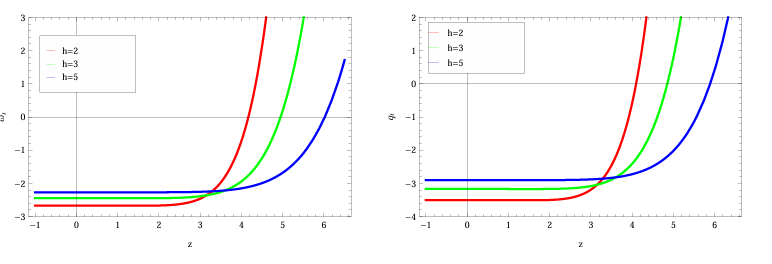
\includegraphics[width=1.0\textwidth]{fig/fig11.png}
    \caption{EoS参数 $\omega_t$ 和衰减参数 $q_t$ 与 $z$ 的关系}
\end{figure}

$$
\begin{aligned}
    f_{TT}
    &=\frac{(1+z)^{4/h} }{36h^4 } \bigg[\frac{3h(3h+2)\kappa^2\rho_{m0} }{2a_0^3(3h+1) }(1+z)^3 + \frac{2h(2h+1)\kappa^2 B_0^2 }{a_0^4(4h+1) } (1+z)^4 \\
    &- \frac{32h(4h+1)\kappa^2 B_0^4 \omega_0 }{a_0^8 (8h+1) } (1+z)^8 - \frac{c_1 }{4(1+z)^{1/h} }   \bigg].
\end{aligned}
$$
\begin{figure}
    \centering
    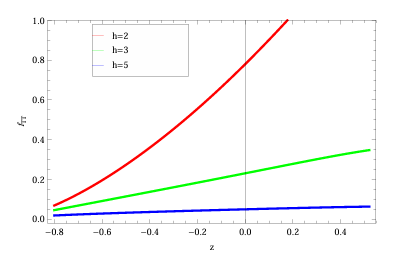
\includegraphics[width=0.6\textwidth]{fig/fig12.png}
    \caption{$f_{TT}$ 与 $z$ 的关系}
\end{figure}

$$
\begin{aligned}
    &\frac{\mathrm{d}S_H }{\mathrm{d}t } + \frac{\mathrm{d}S_I }{\mathrm{d}t } \\
    =&-\frac{\pi(1+z)^{3/h} }{Gh^3 } \bigg[\frac{3h(3h+4)\kappa^2\rho_{m0} }{2a_0^3(3h+1) }(1+z)^3 + \frac{4(h+1)\kappa^2 B_0^2 }{3a_0^4(4h+1) } (1+z)^4 \\
    &- \frac{64h(2h+1)\kappa^2 B_0^4 \omega_0 }{3a_0^8 (8h+1) } (1+z)^8- \frac{c_1 }{4h(1+z)^{1/h} } \bigg] + \frac{2\pi }{G h^3 } (1+h)(1+z)^{1/h}.
\end{aligned}
$$

$$
\begin{aligned}
    &\frac{\mathrm{d}S_E }{\mathrm{d}t } + \frac{\mathrm{d}S_I }{\mathrm{d}t } \\
    =&-\frac{\pi(1+z)^{3/h} }{Gh(1+h)^2 } \bigg[\frac{(3h+4)\kappa^2\rho_{m0} }{2a_0^3(3h+1) }(1+z)^3 + \frac{4(h+1)\kappa^2 B_0^2 }{3a_0^4(4h+1) } (1+z)^4 \\
    &- \frac{64(2h+1)\kappa^2 B_0^4 \omega_0 }{3a_0^8 (8h+1) } (1+z)^8 - \frac{c_1 }{4h\kappa^2(1+z)^{1/h} } \bigg] + \frac{2\pi h }{G (1+h)^3 } (1+z)^{1/h}
\end{aligned}
$$

\begin{figure}
    \centering
    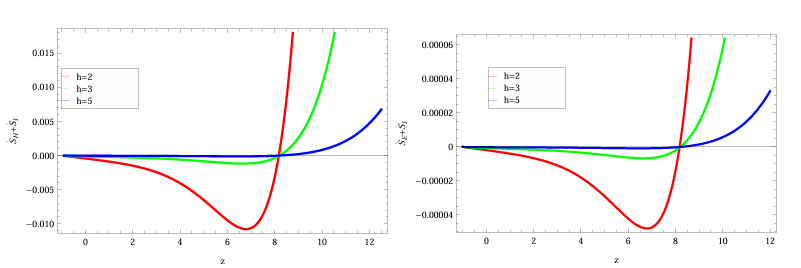
\includegraphics[width=0.7\textwidth]{fig/fig13.png}
    \caption{$\dot{S}_H+\dot{S}_I$,left for Hubble Horizon,right for Event Horizon}
\end{figure}


$a(t)=a_0(t_s-t)^h$,与之对应的 $f(T)$ 模型
    
$$
\begin{aligned}
    f(T)
    &=c_2\left(-\frac{T }{6h^2 }  \right)^{1/2} + \frac{2\kappa^2\rho_{m0} }{a_0^3(1-3h) } \left(-\frac{T }{6h^2 }  \right)^{3h/2} + \frac{\kappa^2 B_0^2 }{a_0^4(1-4h) } \left(-\frac{T }{6h^2 }  \right)^{2h} \\
    &- \frac{8\kappa^2 B_0^4 \omega_0 }{a_0^8(1-8h) } \left(-\frac{T }{6h^2 }  \right)^{4h},
\end{aligned}
$$
\begin{figure}
    \centering
    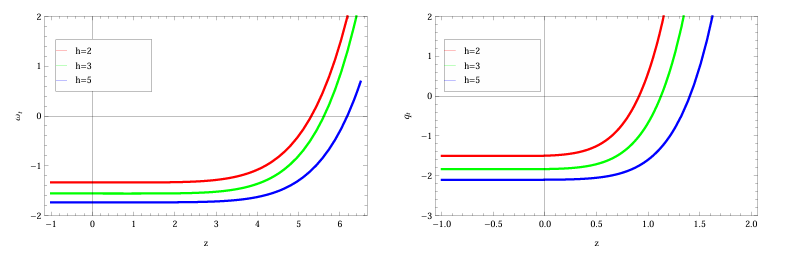
\includegraphics[width=0.7\textwidth]{fig/fig14.png}
    \caption{另一种尺度因子的 $\omega_t$ 和 $q_t$}
\end{figure}

\begin{figure}
    \centering
    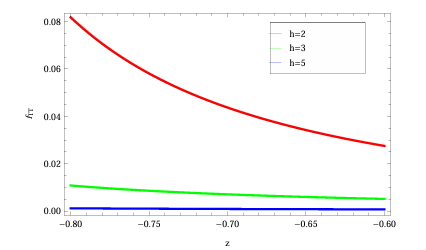
\includegraphics[width=0.6\textwidth]{fig/fig15.png}
    \caption{另一种尺度因子的 $f_{TT}$}
\end{figure}
\begin{figure}[H]
    \centering
    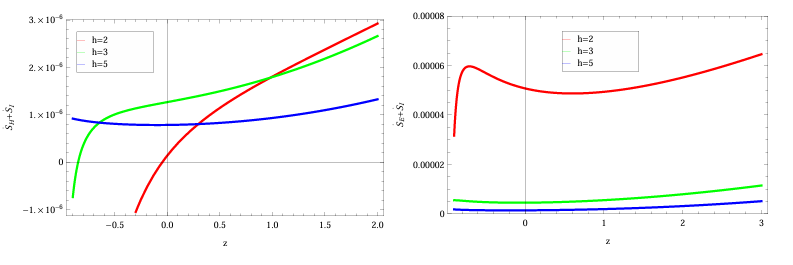
\includegraphics[width=0.6\textwidth]{fig/fig16.png}
    \caption{另一种尺度因子的 $\dot{S}_H+\dot{S}_I$,left for Hubble Horizon,right for Event Horizon}
\end{figure}

\subsection{4. 小结}

本文在包含暗能量、尘埃物质和磁场贡献的 FRW 宇宙中,在 f(T) 引力框架下研究了 NLED。采用平均手段来保留 NLED 中时空的各向同性。在这种情况下,评估了宇宙总能量密度和压力的 EoS 和减速参数。开发了哈勃和事件视界的总熵的时间导数,以使用视界熵和吉布斯方程来研究 GSLT 的合法性(validity)。使用极点和幂律形式的尺度因子构建了 f(T) 模型。讨论了一些特定模型参数的图形行为。文章的结果总结如下:

\begin{itemize}
    \item 第一个由极点尺度因子构建的 f(T) 模型的宇宙学参数代表一个在 z≤5.6 时加速膨胀的 phamtom dominated 的宇宙。对于更高的 z 值,膨胀率降低,磁场主导扭率贡献,代表减速膨胀的宇宙。
    \item 作了哈勃和事件视界的总熵的时间导数关于 $z$ 的图,以讨论 GSLT 对满足条件 $f_{TT} \ll 1 $  的模型的合法性。对于这两个视界,GSLT 对 $z >8.2$ 和 $z <0$ 都成立。
    \item 使用精确幂律比例因子构建第二个 $f(T)$ 模型。$\omega_t$ 和 $q_t$ 关系 $z$ 的关系图表明与第一个模型相同的行为。
    \item 第二个模型也满足条件 $f_{TT}\ll 1$,以借助热力学第一定律讨论 GSLT。图6显示了哈勃视界总熵的时间导数在 $h = 2,3$ 时 $z$ 的一定范围内的正行为,而 $h = 5$ 表示 GSLT 对所有 $z$ 值的合法性。对于事件视界,GSLT 对所有 $h$ 和 $z$ 值都合法。
    \item 值得一提的是,仅对于磁宇宙,当 $z > -0.1$ 时,事件视界的总熵的时间变化率保持正值,在此范围之外变为负值。另一方面,在我们的例子中,对于具有幂律比例因子的视界,它对于磁 f(T) 框架中的所有 $z$ 值都保持在正区域。哈勃视界在两种情况下都表现出总熵的时间导数的相似行为。对于更高的红移值,宇宙学参数表明,与磁场相比,扭转贡献变得微弱。它指向宇宙的早期减速阶段。
\end{itemize}

\section{V. 总结}

本文综合了三篇关于非线性电动力学(NLED)的研究,探讨了其在平坦时空中、与引力耦合的黑洞解以及在f(T)引力理论中的应用。这些研究展示了NLED在解决经典电动力学和广义相对论中奇点问题的潜力,同时也揭示了其在宇宙学中的重要应用前景。

首先,Anjan Kar的研究提出了一种新的NLED模型,该模型在平坦时空中表现出有限的点电荷电场和自能,并在与引力耦合时能够产生正则黑洞或裸奇点解。这一模型在弱场极限下与Born-Infeld电动力学相似,但在强场极限下表现出独特的性质。研究表明,该模型在平坦时空中能够消除点电荷的无限自能问题,并在与引力耦合时产生无奇点的黑洞解。然而,该模型在磁性场的因果性和能量条件方面仍面临一些挑战。

其次,N. Bretón和R. García-Salcedo的研究回顾了NLED在黑洞物理中的应用,特别是Born-Infeld电动力学与引力耦合的解。研究表明,Born-Infeld理论能够产生无奇点的黑洞解,并在某些情况下表现出与Reissner-Nordström解类似的渐近行为。然而,这些解在能量条件和稳定性方面仍存在争议。此外,研究还探讨了NLED黑洞的热力学性质,发现其满足黑洞力学的第一定律,但Smarr公式需要进行修正。

最后,M. Sharif和Shamaila Rani的研究探讨了NLED在f(T)引力理论中的应用,特别是在宇宙加速膨胀和广义第二定律(GSLT)的有效性方面。研究表明,NLED在f(T)引力理论中能够产生与宇宙加速膨胀一致的解,并在某些情况下满足GSLT。通过构造具体的f(T)模型,研究发现NLED在宇宙早期阶段能够避免初始奇点,并在晚期阶段表现出标准的辐射相。

综上所述,NLED在解决经典电动力学和广义相对论中的奇点问题方面表现出巨大潜力,但在引力耦合和宇宙学应用中仍面临诸多挑战。未来的研究需要进一步探索NLED在不同物理背景下的行为,并解决其在能量条件和稳定性方面的潜在问题。

% Put \label in argument of \section for cross-referencing
%\section{\label{}}
\subsection{}
\subsubsection{}

% If in two-column mode, this environment will change to single-column
% format so that long equations can be displayed. Use
% sparingly.
%\begin{widetext}
% put long equation here
%\end{widetext}

% figures should be put into the text as floats.
% Use the graphics or graphicx packages (distributed with LaTeX2e)
% and the \includegraphics macro defined in those packages.
% See the LaTeX Graphics Companion by Michel Goosens, Sebastian Rahtz,
% and Frank Mittelbach for instance.
%
% Here is an example of the general form of a figure:
% Fill in the caption in the braces of the \caption{} command. Put the label
% that you will use with \ref{} command in the braces of the \label{} command.
% Use the figure* environment if the figure should span across the
% entire page. There is no need to do explicit centering.

% \begin{figure}
% \includegraphics{}%
% \caption{\label{}}
% \end{figure}

% Surround figure environment with turnpage environment for landscape
% figure
% \begin{turnpage}
% \begin{figure}
% \includegraphics{}%
% \caption{\label{}}
% \end{figure}
% \end{turnpage}

% tables should appear as floats within the text
%
% Here is an example of the general form of a table:
% Fill in the caption in the braces of the \caption{} command. Put the label
% that you will use with \ref{} command in the braces of the \label{} command.
% Insert the column specifiers (l, r, c, d, etc.) in the empty braces of the
% \begin{tabular}{} command.
% The ruledtabular enviroment adds doubled rules to table and sets a
% reasonable default table settings.
% Use the table* environment to get a full-width table in two-column
% Add \usepackage{longtable} and the longtable (or longtable*}
% environment for nicely formatted long tables. Or use the the [H]
% placement option to break a long table (with less control than 
% in longtable).
% \begin{table}%[H] add [H] placement to break table across pages
% \caption{\label{}}
% \begin{ruledtabular}
% \begin{tabular}{}
% Lines of table here ending with \\
% \end{tabular}
% \end{ruledtabular}
% \end{table}

% Surround table environment with turnpage environment for landscape
% table
% \begin{turnpage}
% \begin{table}
% \caption{\label{}}
% \begin{ruledtabular}
% \begin{tabular}{}
% \end{tabular}
% \end{ruledtabular}
% \end{table}
% \end{turnpage}

% Specify following sections are appendices. Use \appendix* if there
% only one appendix.
%\appendix
%\section{}

% If you have acknowledgments, this puts in the proper section head.
%\begin{acknowledgments}
% put your acknowledgments here.
%\end{acknowledgments}

% Create the reference section using BibTeX:
\bibliography{ref.bib}

\end{document}
%
% ****** End of file apstemplate.tex ******

